%%%%%%%%%%%%%%%%%%%%%%%%%%%%%%%%%%%%%%%%%%%%%%%%%%%%%%%%%%%%%%%%%%%%%%%%
% Dual-Stream Aerial Detection Conference Paper (ICSPIS 2026)
% IEEE Conference Template (Two-Column, Strictly <= 6 Pages)
%%%%%%%%%%%%%%%%%%%%%%%%%%%%%%%%%%%%%%%%%%%%%%%%%%%%%%%%%%%%%%%%%%%%%%%%
\documentclass[conference]{IEEEtran}
\IEEEoverridecommandlockouts

\usepackage{cite}
\usepackage{amsmath,amssymb,amsfonts}
\usepackage{algorithm}
\usepackage{algorithmic}
\usepackage{graphicx}
\usepackage{textcomp}
\usepackage{xcolor}
\usepackage{booktabs}
\usepackage{url}
\usepackage{balance}
\usepackage{placeins}
\usepackage{tikz}
\usepackage{pgfplots}

\pgfplotsset{compat=1.18}
\usetikzlibrary{arrows.meta,positioning,shapes.geometric,calc,fit,backgrounds,decorations.pathreplacing,plotmarks,patterns}

% Declare custom pentagon* plotmark used in figure_performance_tradeoff.tex
\pgfdeclareplotmark{pentagon*}{%
  \pgfpathmoveto{\pgfpointpolar{90}{\pgfplotmarksize}}%
  \pgfpathlineto{\pgfpointpolar{162}{\pgfplotmarksize}}%
  \pgfpathlineto{\pgfpointpolar{234}{\pgfplotmarksize}}%
  \pgfpathlineto{\pgfpointpolar{306}{\pgfplotmarksize}}%
  \pgfpathlineto{\pgfpointpolar{18}{\pgfplotmarksize}}%
  \pgfpathclose
  \pgfusepathqfillstroke
}

\setlength{\textfloatsep}{4pt plus 1pt minus 1pt}
\setlength{\floatsep}{3pt plus 1pt minus 1pt}
\setlength{\intextsep}{3pt plus 1pt minus 1pt}
\setlength{\abovecaptionskip}{2pt plus 1pt minus 1pt}
\setlength{\belowcaptionskip}{1pt plus 1pt minus 1pt}

\setcounter{topnumber}{4}
\setcounter{bottomnumber}{4}
\setcounter{totalnumber}{6}
\setcounter{dbltopnumber}{4}
\renewcommand{\topfraction}{0.95}
\renewcommand{\bottomfraction}{0.95}
\renewcommand{\textfraction}{0.05}
\renewcommand{\floatpagefraction}{0.85}
\renewcommand{\dbltopfraction}{0.95}
\renewcommand{\dblfloatpagefraction}{0.85}

\begin{document}

\title{Causal Temporal Filtering for Reliable Alerts in Dual-Stream UAV Search and Rescue Detection}
\author{\IEEEauthorblockN{1\textsuperscript{st} Oumar Mamoun Ibrahim}
\IEEEauthorblockA{\textit{Department of Computer Engineering} \\
\textit{University of Sharjah}\\
Sharjah, UAE \\
U22200741@sharjah.ac.ae}
\and
\IEEEauthorblockN{2\textsuperscript{nd} Mohamad Khairi bin Ishak}
\IEEEauthorblockA{\textit{Department of Computer Engineering} \\
\textit{University of Sharjah}\\
Sharjah, UAE \\
mishak@sharjah.ac.ae} 
}

\maketitle

\begingroup
\renewcommand\thefootnote{}
\footnotetext{Ethical Statement: No living human subjects or animals were involved in this research; all video streams were synthetically generated using generative models. The authors confirm that all experimental procedures and protocols are exempt from review board approval. Code, simulation frameworks, and dataset split manifests are publicly available at: \url{https://github.com/IamOumarIbrahim/multi-modal-detection}.}
\endgroup

\begin{abstract}
Autonomous unmanned aerial vehicles in wilderness search and rescue require reliable alerts under strict size, weight, power, and cost constraints. In these missions, temporary detector noise triggers costly hover maneuvers that waste battery life. In this paper, we evaluate causal temporal decision strategies to convert noisy dual-stream detections into reliable alerts, focusing primarily on false-alert suppression and alert recall. Across desert, forest, and alpine biomes with synchronized visible and pseudo-thermal video streams, fixed YOLO11n detectors feed a late-fusion max gate and a five-frame sliding window spanning 166.7 milliseconds at 24 frames per second. We evaluate raw thresholding, moving average, median filtering, history consensus, a Mamba selective state-space model, and a gated recurrent unit. Learned sequence models achieve the strongest overall false-alert suppression and high alert recall: Mamba yields the fewest false alerts at 1.7 per minute with 87.7\% tile recall, while the gated recurrent unit achieves 86.2\% tile recall and the highest frame $F_1$-score. In comparison, a training-free moving average reduces false alerts to 2.1 per minute with 84.6\% tile recall, and a median filter preserves 92.3\% tile recall with 3.6 false alerts per minute. Filter latency is negligible across all methods, consuming less than 0.4\% of the frame budget. Therefore, the main engineering trade-off for edge deployment is memory footprint and training requirements rather than execution speed. Simple causal filters offer a lightweight, training-free alternative to learned models.
\end{abstract}

\begin{IEEEkeywords}
edge computing, object detection, search and rescue, temporal filtering, unmanned aerial vehicles.
\end{IEEEkeywords}

\begin{figure*}[!t]
\centering
\resizebox{1.0\textwidth}{!}{\begin{tikzpicture}[
>=Stealth,
font=\sffamily\small,
box/.style={draw=black!70, rounded corners=3pt, thick, fill=white, align=center},
iconbox/.style={draw=none, fill=none, align=center, inner sep=1pt},
videobox/.style={draw=blue!60!black, rounded corners=3pt, thick, fill=black!2, align=center, inner sep=2.5pt},
framebox/.style={draw=teal!60!black, rounded corners=3pt, thick, fill=white, align=center, inner sep=2.5pt},
stepbox/.style={box, fill=green!12, draw=green!60!black, thick, font=\sffamily\scriptsize, align=center},
detector/.style={box, fill=cyan!10, draw=cyan!70, font=\sffamily\footnotesize, text width=2.6cm, minimum height=1.15cm},
fusion/.style={box, fill=purple!10, draw=purple!70, thick, font=\sffamily\footnotesize, text width=2.5cm, minimum height=1.1cm},
method/.style={box, fill=orange!10, draw=orange!75, thick, font=\sffamily\scriptsize, text width=3.7cm, inner ysep=5pt, inner xsep=7pt},
decision/.style={box, fill=teal!12, draw=teal!70, thick, font=\sffamily\footnotesize, text width=2.2cm, minimum height=1.05cm},
eval/.style={box, fill=green!10, draw=green!60!black, thick, font=\sffamily\scriptsize, text width=3.4cm, inner ysep=4.5pt, inner xsep=5pt},
kpi/.style={draw=red!70!black, fill=red!5, rounded corners=4pt, thick, align=center, inner ysep=4.5pt, inner xsep=5pt, text width=3.2cm},
arrow/.style={->, thick, draw=black!75},
bluearrow/.style={->, thick, draw=blue!70!black},
orangearrow/.style={->, thick, draw=orange!80!black},
greenarrow/.style={->, thick, draw=green!60!black},
purplearrow/.style={->, thick, draw=purple!80!black},
sig/.style={font=\fontsize{5.8pt}{6.8pt}\selectfont\bfseries, text=black},
ttl/.style={font=\fontsize{6.2pt}{7.2pt}\selectfont\bfseries}
]

% =========================================================================
% TOP SECTION: SYNTHETIC GENERATION, DUAL CROP & ANNOTATION
% =========================================================================

% 1. RGB video prompt
\node[iconbox] (prompt_rgb) at (-4.6, 6.10) {

\includegraphics[height=0.76cm]{figures/icon_lorem_ipsum.png}
};
\node[above=4pt of prompt_rgb, ttl, text=blue!80!black] (lbl_p1) {Scenario Prompt};
\node[below=2pt of prompt_rgb, font=\fontsize{5.3pt}{6.4pt}\selectfont\bfseries, text=black] (sub_p1) {Structured Text};

% 2. Video Generator LLMs
\node[iconbox] (grok_rgb) at (-1.4, 7.35) {

\includegraphics[height=0.72cm]{figures/grok_logo.png}
};
\node[above=3pt of grok_rgb, ttl, text=purple!80!black] (lbl_g1) {AI Video Generator};
\node[below=2pt of grok_rgb, font=\fontsize{5.3pt}{6.4pt}\selectfont\bfseries, text=black] (sub_grok) {xAI Grok};

\node[iconbox] (gemini_rgb) at (-1.4, 4.85) {

\includegraphics[height=0.72cm]{figures/gemini_logo.png}
};
\node[below=2pt of gemini_rgb, font=\fontsize{5.3pt}{6.4pt}\selectfont\bfseries, text=black] (sub_g1) {Google Gemini 3.8 Flash};

\draw[bluearrow] (prompt_rgb.east) -- (grok_rgb.west);
\draw[bluearrow] (prompt_rgb.east) -- (gemini_rgb.west);

% 3. 16:9 RGB Videos — Snow only in video boxes
\node[videobox] (grok_videos) at (2.6, 7.35) {
\begin{tabular}{@{}c@{\hspace{3pt}}c@{\hspace{3pt}}c@{}}
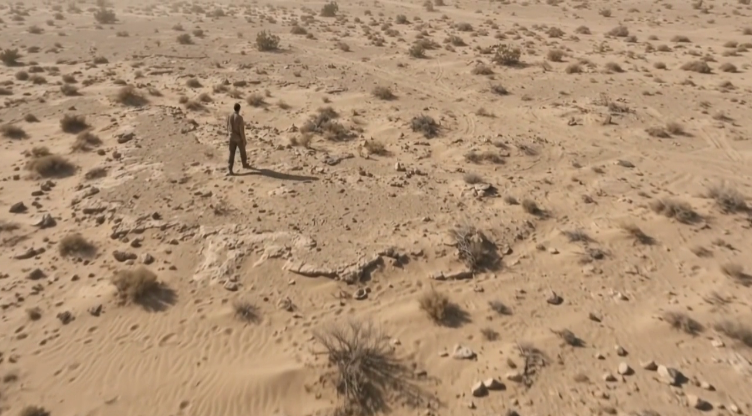
\includegraphics[width=1.12cm]{figures/grok_desert_video.png} &
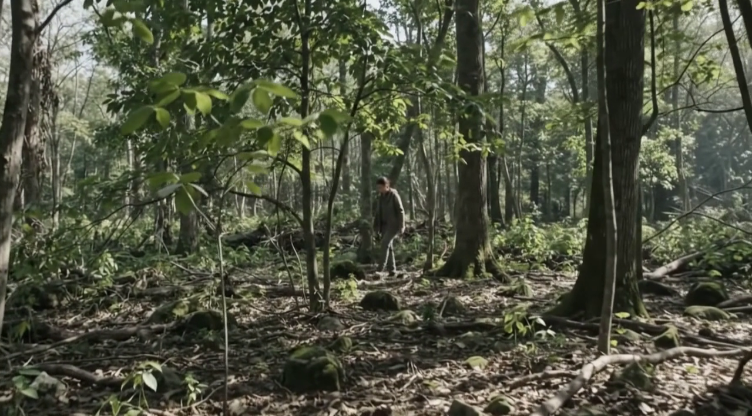
\includegraphics[width=1.12cm]{figures/grok_forest_video.png} &
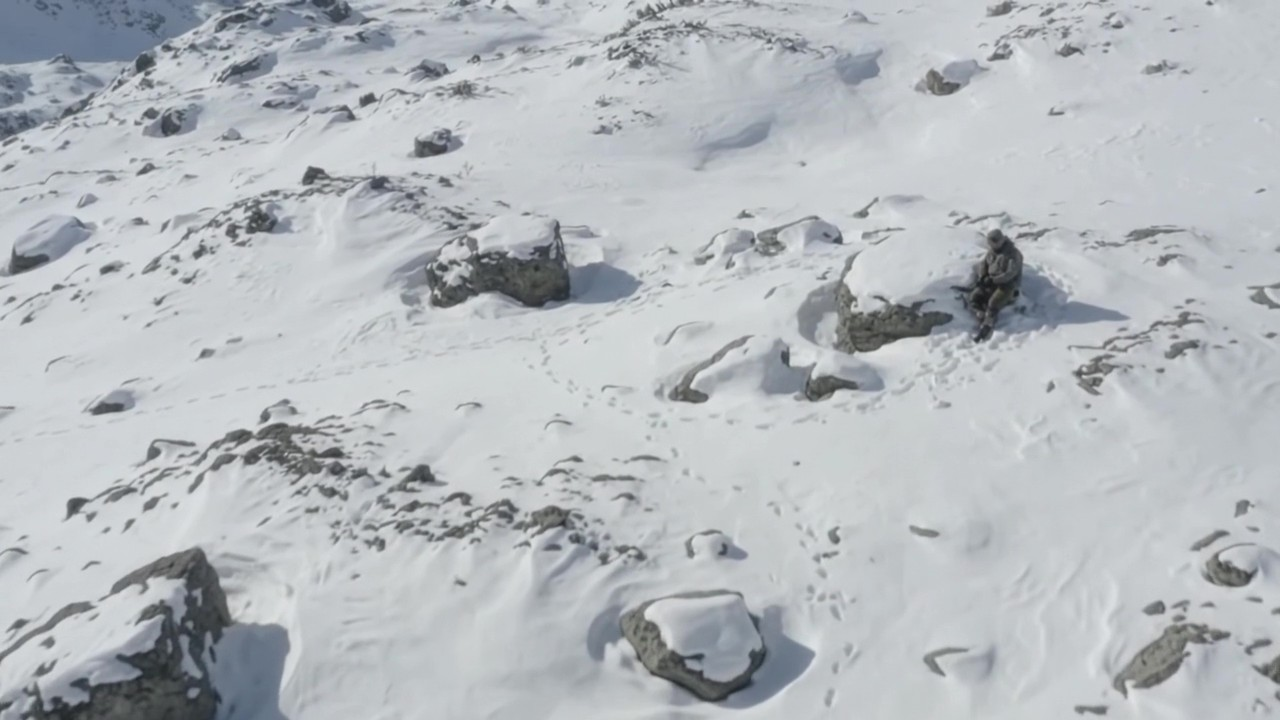
\includegraphics[width=1.12cm]{figures/snow_rgb_video.jpg} \\
{\tiny\bfseries Desert RGB} & {\tiny\bfseries Forest RGB} & {\tiny\bfseries Snow RGB}
\end{tabular}
};
\node[above=3pt of grok_videos, ttl, text=black] (lbl_gv) {16:9 RGB Videos};
\node[below=2pt of grok_videos, font=\fontsize{5.3pt}{6.4pt}\selectfont\bfseries, text=black] (sub_gv) {752$\times$416 @ 24 FPS};

\draw[bluearrow] (grok_rgb.east) -- (grok_videos.west);

\node[videobox] (rgb_videos) at (2.6, 4.85) {
\begin{tabular}{@{}c@{\hspace{3pt}}c@{\hspace{3pt}}c@{}}
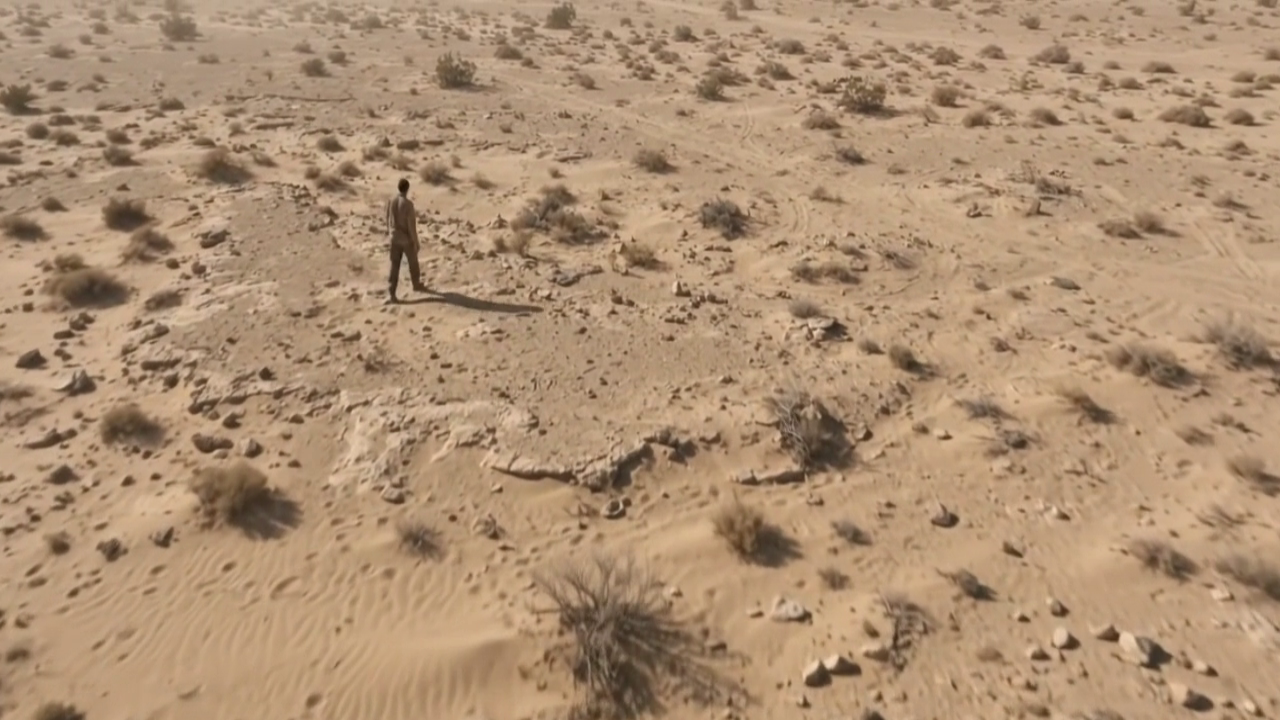
\includegraphics[width=1.12cm]{figures/desert_rgb_video.png} &
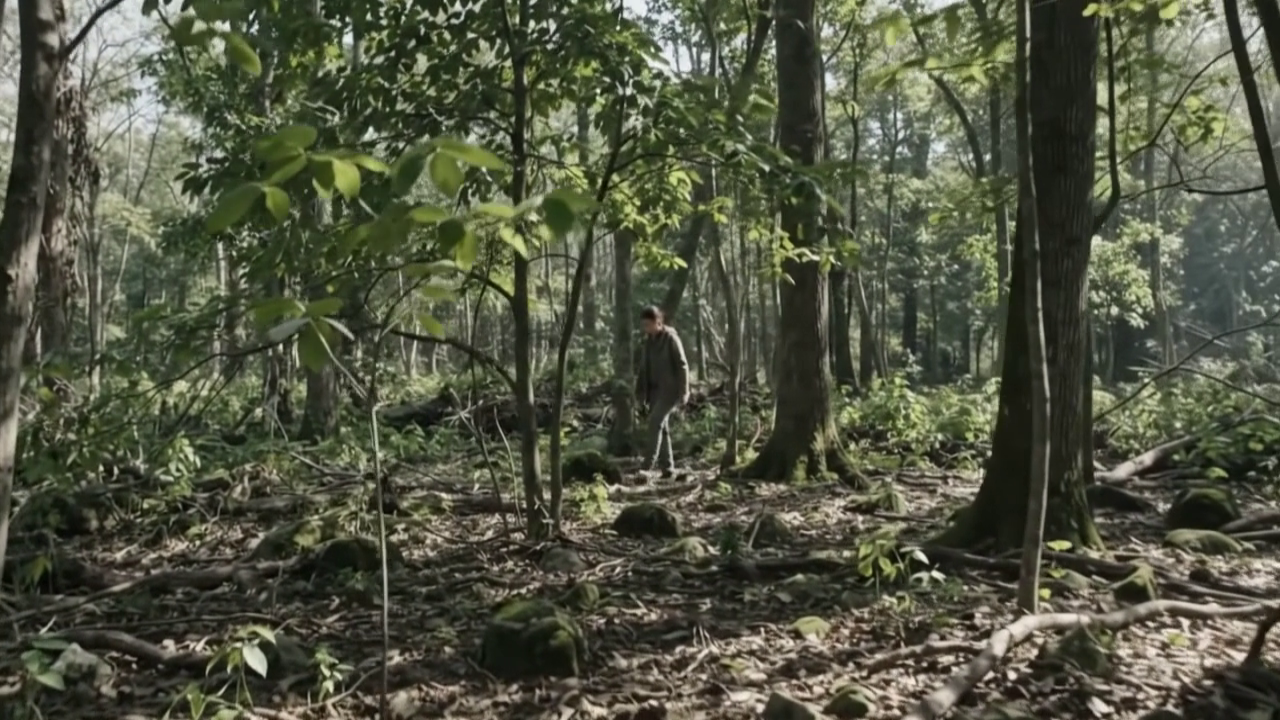
\includegraphics[width=1.12cm]{figures/forest_rgb_video.png} &
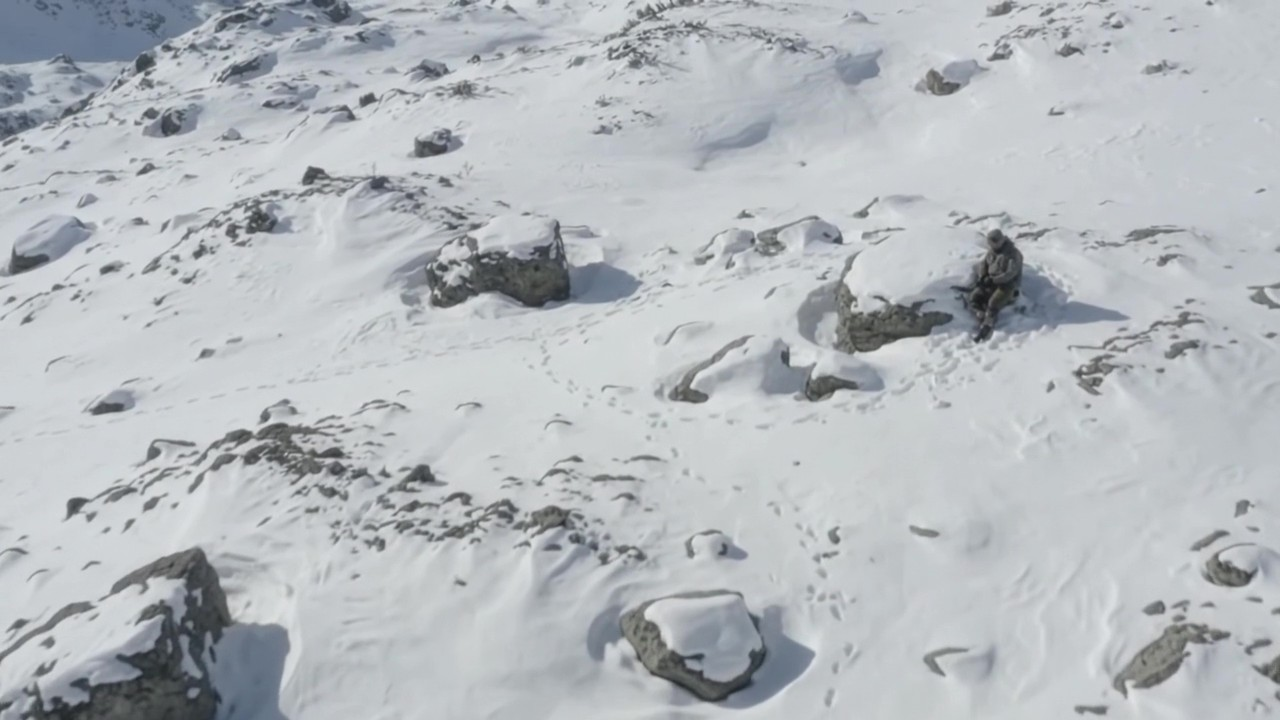
\includegraphics[width=1.12cm]{figures/snow_rgb_video.jpg} \\
{\tiny\bfseries Desert RGB} & {\tiny\bfseries Forest RGB} & {\tiny\bfseries Snow RGB}
\end{tabular}
};
\node[above=3pt of rgb_videos, ttl, text=black] (lbl_v1) {16:9 RGB Videos};
\node[below=2pt of rgb_videos, font=\fontsize{5.3pt}{6.4pt}\selectfont\bfseries, text=black] (sub_v1) {1280$\times$720 @ 24 FPS};

\draw[bluearrow] (gemini_rgb.east) -- (rgb_videos.west);

% 4. Resolution Upscale
\node[box, fill=blue!8, draw=blue!70!black, thick, font=\fontsize{5.6pt}{6.6pt}\selectfont, text width=2.1cm, align=center, minimum height=1.05cm] (upscale_box) at (6.6, 7.35) {
\textbf{Upscale to}\\[1pt]
\textbf{1280$\times$720}\\[2pt]
{\tiny Spatial Scaling}
};
\node[above=3pt of upscale_box, ttl, text=blue!80!black] (lbl_up) {Resolution Upscale};

\draw[bluearrow] (grok_videos.east) -- (upscale_box.west);

% 5. Melo Thermal Stylizing
\node[box, fill=orange!10, draw=orange!80!black, thick, font=\fontsize{5.6pt}{6.6pt}\selectfont, text width=2.6cm, align=center, minimum height=1.15cm] (melo_th) at (10.0, 6.0) {
\textbf{256-Level Color LUT}\\[2pt]
{\scriptsize Grayscale Luminance Remap}\\[1pt]
{\tiny Non-Linear Color Transform}
};
\node[above=4pt of melo_th, ttl, text=orange!80!black] (lbl_melo) {Pseudo-TIR Color Transfer};
\node[below=3pt of melo_th, font=\fontsize{5.3pt}{6.4pt}\selectfont\bfseries, text=black] (sub_melo) {LUT Color Mapping};

\draw[orangearrow] (upscale_box.east) -- ([yshift=5pt]melo_th.west);
\draw[orangearrow] (rgb_videos.east) -- ([yshift=-5pt]melo_th.west);

% 6. 16:9 Thermal Videos
\node[videobox] (th_videos) at (14.5, 6.0) {
\begin{tabular}{@{}c@{\hspace{3pt}}c@{\hspace{3pt}}c@{}}
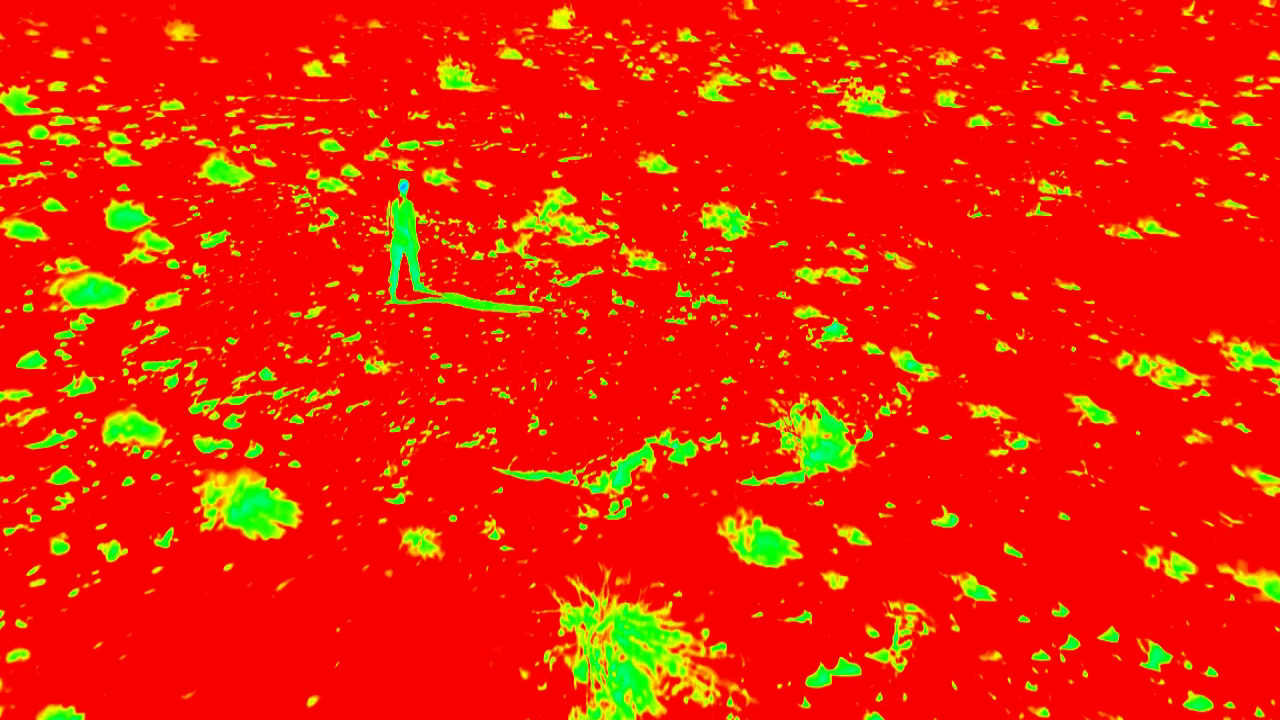
\includegraphics[width=1.12cm]{figures/desert_th_video.png} &
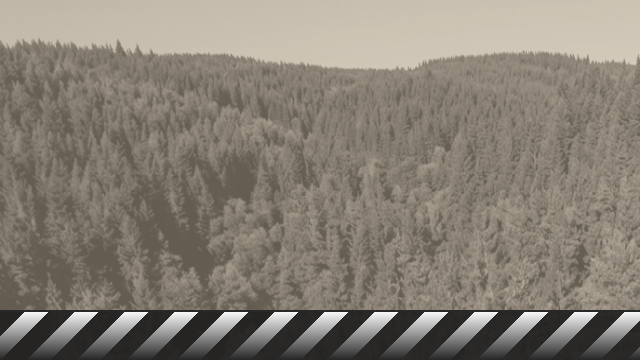
\includegraphics[width=1.12cm]{figures/forest_th_video.png} &
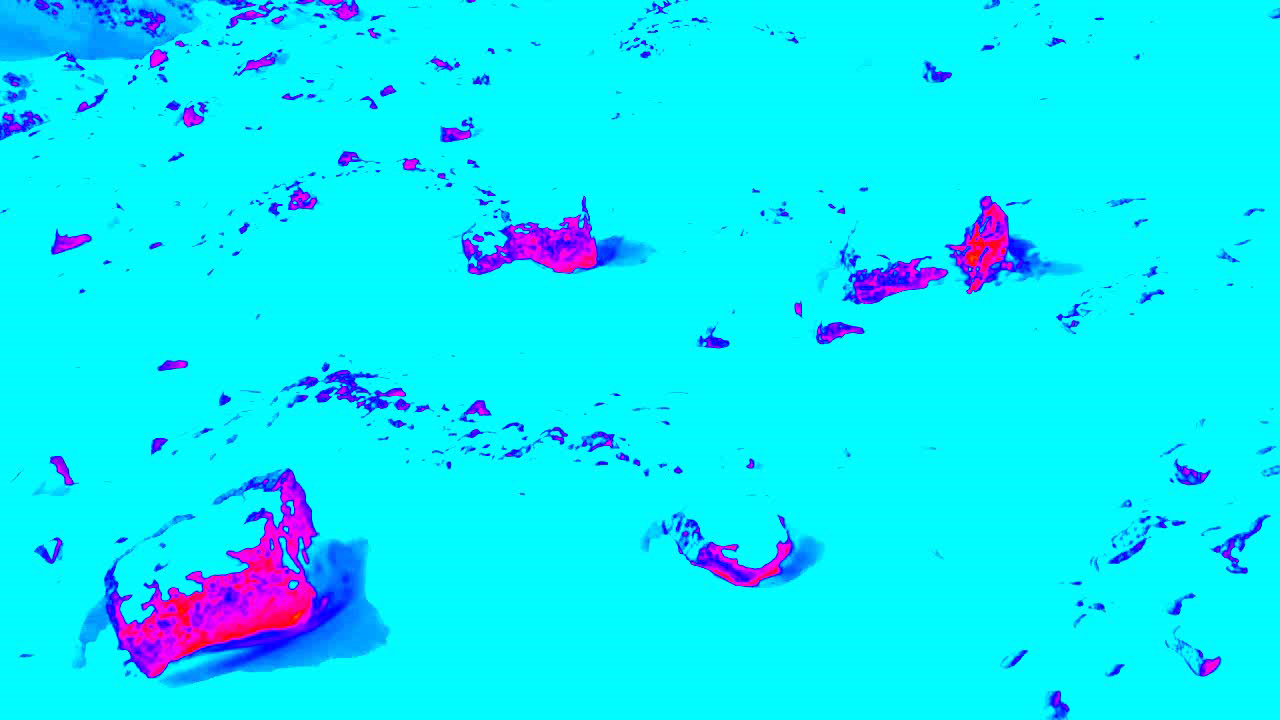
\includegraphics[width=1.12cm]{figures/snow_th_video.jpg.png} \\
{\tiny\bfseries Desert TIR} & {\tiny\bfseries Forest TIR} & {\tiny\bfseries Snow TIR}
\end{tabular}
};
\node[above=4pt of th_videos, ttl, text=black] (lbl_v2) {16:9 Thermal Videos};
\node[below=2pt of th_videos, font=\fontsize{5.3pt}{6.4pt}\selectfont\bfseries, text=black] (sub_v2) {1280$\times$720 @ 24 FPS};

\draw[orangearrow] (melo_th.east) -- (th_videos.west);

% 7. Crop 640x640
\node[videobox] (crops) at (18.5, 6.0) {
\begin{tabular}{@{}c@{\hspace{3pt}}c@{}}
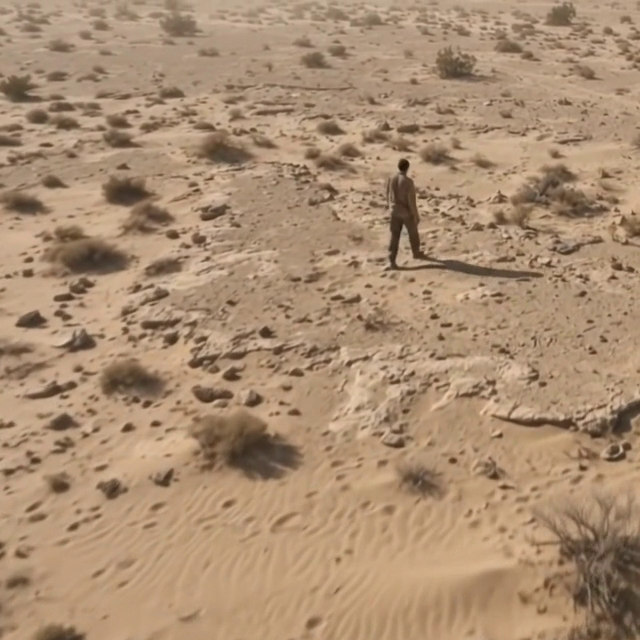
\includegraphics[width=0.83cm]{figures/crop_640_left_video.png} &
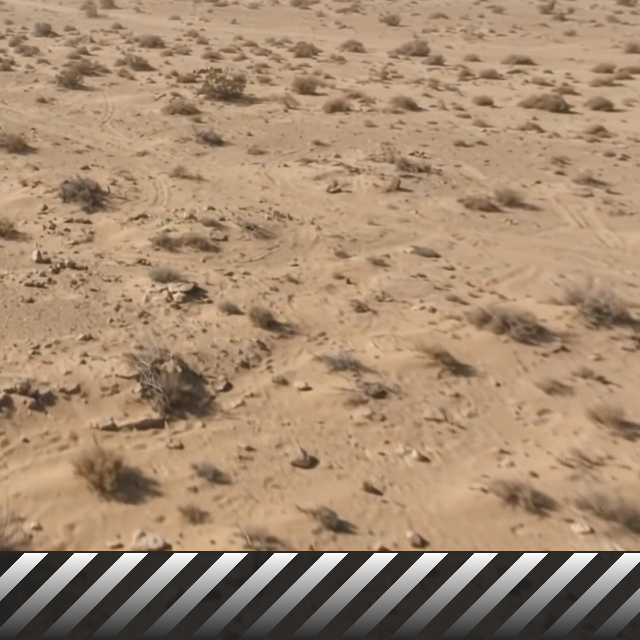
\includegraphics[width=0.83cm]{figures/crop_640_right_video.png} \\
{\tiny\bfseries Left ($x=0$)} & {\tiny\bfseries Right ($x=640$)}
\end{tabular}
};
\node[above=4pt of crops, ttl, text=purple!80!black] (lbl_c) {Crop 640$\times$640 (2 Videos)};
\node[below=2pt of crops, font=\fontsize{5.3pt}{6.4pt}\selectfont\bfseries, text=black] (sub_c) {Cropped Videos (24 FPS)};

\draw[purplearrow] (th_videos) -- (crops);

% 8. Label Studio
\node[iconbox] (label_studio) at (21.6, 6.0) {

\includegraphics[height=0.76cm]{figures/icon_label_studio.png}
};
\node[above=4pt of label_studio, ttl, text=red!80!black] (lbl_ls) {Label Studio};
\node[below=2pt of label_studio, font=\fontsize{5.3pt}{6.4pt}\selectfont\bfseries, text=black] (sub_ls) {Video Annotation};

\draw[purplearrow] (crops) -- (label_studio);

% 9. Video to Frame
\node[stepbox, text width=1.95cm, inner xsep=3pt, minimum height=1.15cm] (v2f) at (24.2, 6.0) {
\textbf{Video to Frame}\\[2pt]
{\scriptsize Full-Rate Stream}\\[-1pt]
{\scriptsize (24~Hz Sampling)}
};
\node[below=2pt of v2f, font=\fontsize{5.3pt}{6.4pt}\selectfont\bfseries, text=black] (sub_v2f) {Frame Extraction};

\draw[greenarrow] (label_studio) -- (v2f);

% 10. Annotated Frames — NO Snow RGB
\node[framebox] (annotated_frames) at (28.0, 6.0) {
\begin{tabular}{@{}c@{\hspace{3pt}}c@{\hspace{3pt}}c@{}}
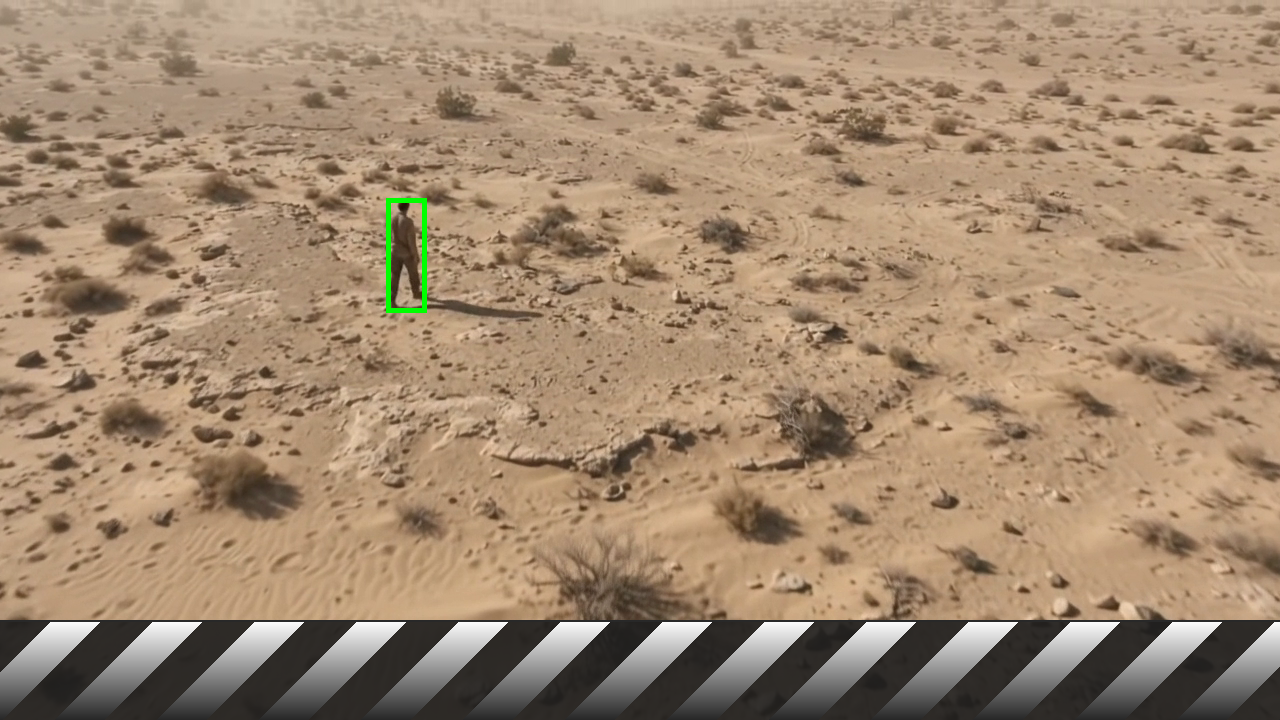
\includegraphics[width=0.82cm]{figures/desert_rgb_annotated.png} &
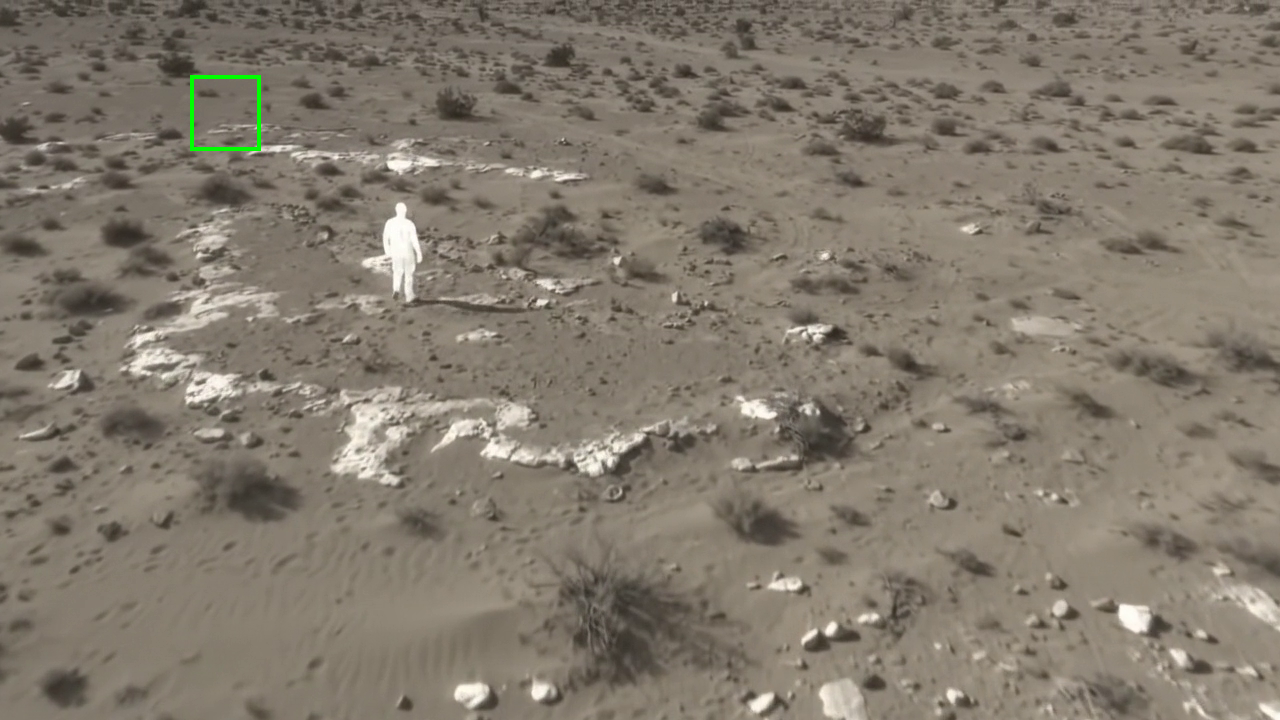
\includegraphics[width=0.82cm]{figures/desert_th_annotated.png} &
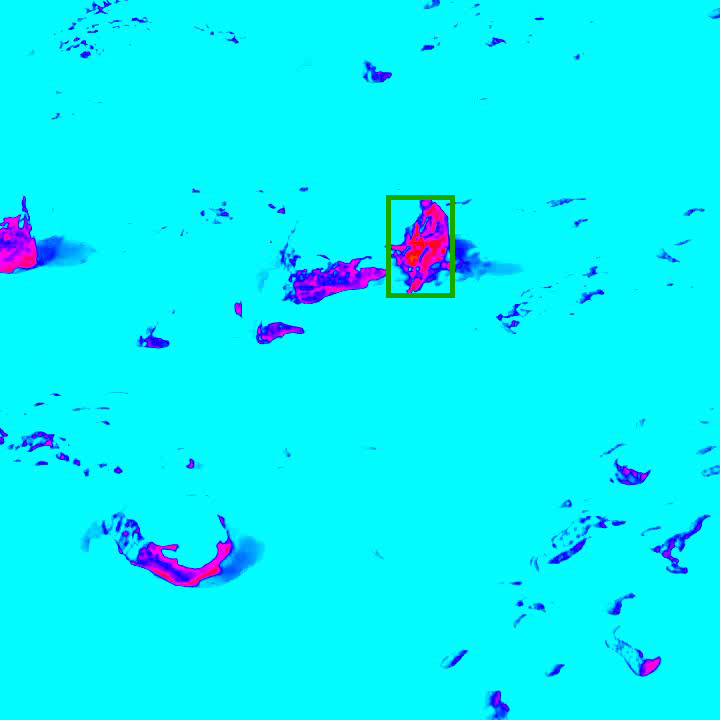
\includegraphics[width=0.82cm]{figures/snow_th_annotated.png} \\
{\tiny\bfseries RGB Frame} & {\tiny\bfseries Thermal Frame} & {\tiny\bfseries Snow TIR}
\end{tabular}
};
\node[above=4pt of annotated_frames, ttl, text=teal!80!black] (lbl_af) {Annotated Frames};
\node[below=2pt of annotated_frames, font=\fontsize{5.3pt}{6.4pt}\selectfont\bfseries, text=black] (sub_af) {Dataset Frames};

\draw[greenarrow] (v2f) -- (annotated_frames);

% =========================================================================
% MIDDLE SECTION: DATASET BANNER
% =========================================================================

\node[draw=purple!70, fill=purple!6, rounded corners=4pt, thick, font=\fontsize{5.8pt}{7.0pt}\selectfont, text=black, inner ysep=4pt, inner xsep=10pt, align=center] (dataset_banner) at (13.5, 3.65) {
\textbf{\textcolor{purple!90!black}{Benchmark Corpus and Sequence Partitioning (Option B)}}\\[2pt]
Parent-Video Grouped Split (44/22/24 tiles $\approx$ 49\%/24\%/27\%) $|$ Co-Located Left and Right Tiles\\
240 Frames/Episode at 24~Hz ($0 \to 239$ Sequential) $|$ Seed 0 Shuffled with Anti-Adjacency
};

\draw[thick, draw=purple!80, ->] (annotated_frames.east) -- ++(0.5, 0) |- (dataset_banner.east);

% =========================================================================
% BOTTOM SECTION: DETECTION, FUSION & POST-PROCESSING
% =========================================================================

\node[box, fill=purple!10, draw=purple!75, thick, font=\fontsize{5.2pt}{6.4pt}\selectfont, text width=1.9cm, align=center] (split_box) at (-1.0, -0.7) {
\textbf{Corpus Split}\\[1pt]
\textbf{Dispatch}\\[2pt]
{\scriptsize Option B Partition}\\[1pt]
{\tiny Shuffled Episodes}
};

\coordinate (split_bus) at (-3.2, 3.65);
\draw[thick, draw=purple!80] (dataset_banner.west) -- node[midway, below=3.5pt, sig, text=purple!90!black] {Curated Dataset Stream} (split_bus);
\draw[arrow, draw=purple!80, thick] (split_bus) |- (split_box.west);

% Detectors
\node[detector] (yolo_rgb) at (3.2, 0.6) {\textbf{RGB Detector}\\[1pt]YOLO11n\\[1pt]{\scriptsize 640$\times$640, 2.6M}\\[-1pt]{\scriptsize Batch: 16, FP32}};
\node[detector] (yolo_tir) at (3.2, -2.0) {\textbf{Thermal Detector}\\[1pt]YOLO11n\\[1pt]{\scriptsize 640$\times$640, 2.6M}\\[-1pt]{\scriptsize Batch: 16, FP32}};

\draw[arrow, blue!70!black, thick] (split_box.north east) to[out=20, in=180] node[pos=0.45, above=4pt, sig] {RGB Input} (yolo_rgb.west);
\draw[arrow, orange!70!black, thick] (split_box.south east) to[out=-20, in=180] node[pos=0.45, below=8pt, sig] {Thermal Input} (yolo_tir.west);

% Late Decision Fusion
\node[fusion] (fusion) at (7.2, -0.7) {
\textbf{Late Decision Fusion}\\[2pt]
Confidence Max Gate\\[2pt]
{\scriptsize Soft Disjunctive OR}
};

\draw[arrow, blue!70!black] (yolo_rgb.east) -- node[pos=0.45, above=4pt, sig] {RGB Score} (fusion.north west);
\draw[arrow, orange!70!black] (yolo_tir.east) -- node[pos=0.65, below=4pt, sig] {Thermal Score} (fusion.south west);

% Causal Post-Processing Methods (M1–M6)
\node[method] (m1) at (13.3, 2.15) {\textbf{M1: Raw Baseline}\\[1pt]Direct Score Threshold\\{\tiny (Instantaneous Confidence)}};
\node[method] (m2) at (13.3, 0.85) {\textbf{M2: Moving Average}\\[1pt]Sliding Window Mean\\{\tiny (5-Frame Window, 166.7 ms span)}};
\node[method] (m3) at (13.3, -0.45) {\textbf{M3: Median Filter}\\[1pt]Order-Statistic Median\\{\tiny (Spike Rejection, 5 Frames)}};
\node[method] (m4) at (13.3, -1.75) {\textbf{M4: History Consensus}\\[1pt]Majority Rule Persistence\\{\tiny (At Least 3 of 5 Detections)}};
\node[method] (m5) at (13.3, -3.05) {\textbf{M5: Learned Mamba-SSSM}\\[1pt]Selective State-Space Filter\\{\tiny (Learned Recurrent Dynamics)}};
\node[method] (m6) at (13.3, -4.45) {\textbf{M6: Learned GRU Baseline}\\[1pt]Single-layer GRU ($d_{\mathrm{h}}=16$)\\{\tiny 1\,681 params, 64\,B state}\\[1pt]
{\tiny Edge-compatible; 44 tiles / 5 seeds}};

% Distribution Bus (extended for M6)
\draw[thick, draw=purple!80] (fusion.east) -- (10.2, -0.7) node[midway, above=4pt, sig, text=purple!90!black] {Fused Score};
\draw[thick, draw=purple!80] (10.2, 2.15) -- (10.2, -4.45);
\draw[arrow, draw=purple!80] (10.2, 2.15) -- (m1.west);
\draw[arrow, draw=purple!80] (10.2, 0.85) -- (m2.west);
\draw[arrow, draw=purple!80] (10.2, -0.45) -- (m3.west);
\draw[arrow, draw=purple!80] (10.2, -1.75) -- (m4.west);
\draw[arrow, draw=purple!80] (10.2, -3.05) -- (m5.west);
\draw[arrow, draw=purple!80] (10.2, -4.45) -- (m6.west);

% Collection Bus (extended for M6)
\draw[thick, draw=teal!80] (16.4, 2.15) -- (16.4, -4.45);
\draw[arrow, draw=teal!80] (m1.east) -- (16.4, 2.15);
\draw[arrow, draw=teal!80] (m2.east) -- (16.4, 0.85);
\draw[arrow, draw=teal!80] (m3.east) -- (16.4, -0.45);
\draw[arrow, draw=teal!80] (m4.east) -- (16.4, -1.75);
\draw[arrow, draw=teal!80] (m5.east) -- (16.4, -3.05);
\draw[arrow, draw=teal!80] (m6.east) -- (16.4, -4.45);

% Alert Decision
\node[decision] (alarm) at (18.9, -0.7) {
\textbf{Alert Decision}\\[2pt]
Verification Gate\\[2pt]
{\scriptsize Optimal Threshold $\tau_m^*$}
};
\draw[arrow, draw=teal!80, very thick] (16.4, -0.7) -- (alarm.west);

% KPI + Evaluation
\node[kpi] (kpi_box) at (23.8, 0.75) {
\textbf{Reliable Alert Generation}\\[1pt]
{\scriptsize False Alert Mitigation (FASR)}\\[-1pt]
{\tiny Filter Buffer Span (166.7~ms)}
};
\coordinate (alarm_split) at (20.6, -0.7);
\draw[thick, draw=teal!80] (alarm.east) -- (alarm_split);
\draw[arrow, draw=red!70!black, thick, rounded corners=5pt] (alarm_split) |- node[pos=0.72, above=5pt, sig, text=red!80!black] {Alarm Stream} (kpi_box.west);

\node[eval] (eval) at (23.8, -1.95) {
\textbf{Operational Evaluation}\\[2pt]
Detection ($R, P, F_1$)\\[1pt]
False Alert Mitigation\\[1pt]
Alert Latency (Table~\ref{tab:postprocessing_benchmark})\\[1pt]
Compute \& Memory Footprint
};
\draw[arrow, draw=blue!70!black, thick, rounded corners=5pt] (alarm_split) |- node[pos=0.72, below=5pt, sig, text=blue!80!black] {Alarm Signal} (eval.west);

\end{tikzpicture}}
\caption{Dual-stream evaluation pipeline with late decision fusion and causal temporal filtering ($W=5$, spanning 166.7~ms at 24~Hz).}
\label{fig:system_architecture}
\end{figure*}

\section{Introduction}

Autonomous unmanned aerial vehicles (UAVs) provide rapid aerial coverage in wilderness search and rescue (SAR) missions \cite{rudol2008human,silvagni2016multipurpose}. Onboard vision systems must operate under strict size, weight, power, and cost (SWaP-C) limits, and remote flights often rely on low-bandwidth telemetry \cite{kyrkou2020emergencynet}. During autonomous flight, false alarms trigger costly hover-and-verify maneuvers that waste battery power and distract operators from search areas.

Optical cameras face different challenges in wilderness environments. Visible red-green-blue (RGB) cameras lose contrast under dense shadows and thick foliage, while real thermal infrared (TIR) cameras detect long-wave radiated heat \cite{hwang2015multispectral,jia2021llvip}. Calibrated radiometric TIR imagery is difficult to generate synthetically at scale. Therefore, we produce a synchronized pseudo-TIR stream using a 256-level grayscale lookup table (LUT) applied to synthetic RGB frames ($Y = 0.299R + 0.587G + 0.114B$). Because this pseudo-TIR channel comes directly from RGB luminance, it contains no independent physical temperature or spectral data. A LUT cannot restore image details lost to deep shadows or bright saturation. Instead, it applies a non-linear luminance mapping that leads convolutional detectors to learn different feature representations. For example, high-reflectance snow and sun-heated desert surfaces appear bright in pseudo-TIR, which is a visual artifact rather than true temperature. We treat this dual-stream setup as a controlled testbed to evaluate how to fuse two correlated edge representations under causal temporal filtering (Section~V-F).

Small UAVs require compact single-stage detectors such as You Only Look Once (YOLO) \cite{redmon2016you}. We use Ultralytics YOLO11n \cite{jocher2024yolo11} (2.6 million parameters, 6.5 giga floating-point operations [GFLOPs] at $640 \times 640$) trained with automatic mixed precision (AMP). However, platform vibration, motion blur, and ground clutter cause per-frame detections to fluctuate, producing temporary false alarms and missed targets.

This problem raises an important systems question: given a fixed, lightweight dual-stream detector, how do learned sequence models and simple causal filters compare in reducing false alerts and preserving recall? Under a 24~Hz video processing budget ($T_s \approx 41.7\text{ ms}$, Eq.~\eqref{eq:realtime_budget}), running two YOLO11n detectors in parallel takes $T_{\text{detect}} \approx 10.2\text{ ms}$ on a GPU ($\sim 40.0\text{ ms}$ on a CPU), while late fusion takes $T_{\text{fusion}} < 0.001\text{ ms}$. In comparison, post-processing filters require only $0.02$ to $150.6\,\mu\text{s}$, which is less than $0.4\%$ of the frame budget. Because even the slowest filter uses roughly 0.4\% of the budget, filter latency does not endanger real-time deadlines, and the drone does not fly past the target. Rather than latency, the primary edge trade-offs are overall false-alert reduction, alert recall, memory footprint, and training data requirements. In our pipeline, confidence scores are merged via late fusion (Section~III) and evaluated using fixed per-method decision thresholds, with zero tuning on the test set (Section~III-C).

This work provides three primary contributions:
\textit{1) Causal Decision Benchmark and Operating Points:} We evaluate six causal decision rules on a fixed dual-stream pipeline, identifying practical operating points for false-alert reduction and recall preservation (Table~\ref{tab:postprocessing_benchmark}, Fig.~\ref{fig:performance_tradeoff});
\textit{2) Analysis of Learned Models vs.\ Classical Filters:} We show that Mamba-SSSM achieves the lowest overall false-alert rate (1.7 FA/min) with high recall, while classical filters achieve competitive reliability with minimal memory state (5--20~B vs.\ 64--512~B) and zero training overhead, identifying memory footprint rather than filter latency as the primary edge differentiator (Section~V-C); and
\textit{3) Dual-Stream Benchmark and Sensitivity Analysis:} We provide a controlled $3\times 2$ evaluation across desert, forest, and snow biomes under parent-video isolation, including recall-weighted $F_2$ and asymmetric-cost sensitivity analyses (Section~V-G).

\section{Related Work}

Multi-sensor aerial vision combines visible and thermal cameras to handle challenging outdoor environments, as explored on ground datasets including KAIST \cite{hwang2015multispectral} and LLVIP \cite{jia2021llvip}. For wilderness SAR, the WiSARD dataset \cite{broyles2022wisard} provides multi-viewpoint benchmarks, while Rudol and Doherty \cite{rudol2008human} demonstrated dual-band geolocation from UAVs. Onboard UAV deployment remains constrained by SWaP-C limits \cite{silvagni2016multipurpose}, because large neural networks quickly drain battery reserves \cite{lygouras2019unsupervised}. Single-stage detectors such as YOLO11n \cite{jocher2024yolo11} achieve real-time frame rates, but detections fluctuate due to camera motion blur and terrain clutter \cite{portmann2014people}, triggering unnecessary hover maneuvers.
 
Classical sequential detection handles signal fluctuations using statistical methods. These include Wald's sequential probability ratio test \cite{wald1945sequential}, radar sliding-window binary integration ($M$-of-$N$) \cite{richards2014fundamentals}, and running median or moving average filters \cite{rabiner1975applications}. More recently, selective state-space models such as Mamba \cite{gu2024mamba} enable sequence modeling with linear computational complexity. Existing SAR literature focuses mainly on per-frame bounding box accuracy. However, previous work does not examine whether learned sequence models are truly needed to convert scalar confidence streams into reliable alerts within edge latency budgets. We address this gap through a direct benchmark on fixed dual-stream outputs.

\section{Methodology}

Our system combines dual-spectrum detection, late fusion, and causal temporal filtering (Fig.~\ref{fig:system_architecture}). Synchronized visible RGB frames $I_{\text{RGB}}[n]$ and pseudo-TIR frames $I_{\text{Thermal}}[n]$ produce per-frame target confidence scores $c_{\text{RGB}}[n], c_{\text{Thermal}}[n] \in [0.0, 1.0]$. The upstream detectors and the late-fusion gate remain fixed in all experiments, so only the temporal filtering method varies.

\subsection{Video Ingestion and Real-Time Edge Budget}
Video streams are processed at $f_s = 24\text{ Hz}$ ($T_s \approx 41.7\text{ ms}$). To avoid dropped frames or buffer delays, total pipeline processing must satisfy:
\begin{equation}
T_{\text{detect}} + T_{\text{fusion}} + T_{\text{filter}} \le 41.7\text{ ms},
\label{eq:realtime_budget}
\end{equation}
where $T_{\text{detect}} = \max(T_{\text{RGB}}, T_{\text{Thermal}})$ is the parallel detection runtime, $T_{\text{fusion}}$ is the fusion latency, and $T_{\text{filter}}$ is the post-processing filter latency. We run two parallel YOLO11n models \cite{jocher2024yolo11}: \textbf{YOLO11n-RGB} and \textbf{YOLO11n-Thermal}. For each frame $n$, the detector yields a scalar confidence score $c[n] = \max_i c_i[n]$ using the highest confidence across all predicted bounding boxes, or $c[n] = 0.0$ if no target is detected. On a desktop GPU, parallel YOLO11n inference takes $T_{\text{detect}} \approx 10.2\text{ ms}$ ($\sim 40.0\text{ ms}$ on CPU), scalar late fusion takes $T_{\text{fusion}} < 0.001\text{ ms}$, and temporal filter execution takes between $0.02\,\mu\text{s}$ and $150.6\,\mu\text{s}$. Total pipeline execution is approximately $10.35\text{ ms}$, which remains well within the 41.7~ms frame deadline ($10.35\text{ ms} \ll 41.7\text{ ms}$).

\subsection{Late Fusion Max Gate}
To combine detections from both visual representations, confidence scores are merged using a late-fusion max gate:
\begin{equation}
s[n] = \max\big(c_{\text{RGB}}[n], \, c_{\text{Thermal}}[n]\big) \in [0.0, 1.0].
\label{eq:late_fusion}
\end{equation}
This disjunctive gate forwards target detections whenever either detector fires with high confidence, without requiring spatial pixel registration. However, it also passes single-stream false-positive spikes, which motivates downstream temporal filtering.

\subsection{Causal Temporal Post-Processing Methods}
Direct thresholding of raw confidence values causes frequent false alarms from temporary clutter spikes. Downstream filters instead buffer confidence scores into a causal sliding window vector of length $W$:
\begin{equation}
\mathbf{w}[n] = \big[s[n-W+1], \, s[n-W+2], \, \dots, \, s[n]\big]^T \in [0.0, 1.0]^W.
\label{eq:window_vector}
\end{equation}
For a nominal window length of $W = 5$, the time span between the earliest and latest buffered frames is $T_{\text{span}} = (W-1)T_s = 166.7\text{ ms}$ ($W T_s = 208.3\text{ ms}$ total integration time). The buffering delay $T_{\text{buffer}} = 166.7\text{ ms}$ is distinct from operational Alert Latency (Section~III-D), which also includes the time needed for detector confidence to ramp up.

Each decision method $m$ uses one fixed threshold $\tau_m^*$ (Table~\ref{tab:postprocessing_benchmark}), shared across all biomes and frozen before the held-out test split is evaluated.
Each $\tau_m^*$ is selected on the \emph{validation} split by sweeping $\tau \in [0.05, 0.95]$ (step $0.02$) and choosing the value that maximises $F_2$ subject to a precision floor $P(\tau) \ge 0.95$, ensuring the recall-heavy cost is penalised without sacrificing operating reliability (see \texttt{scripts/fbeta\_threshold\_sensitivity.py}).
For operational sensitivity analysis (Section~V-G), we also calibrate recall-weighted thresholds with a validation precision floor $P(\tau) \ge 0.95$ under two formulations:
\begin{equation}
\begin{aligned}
\tau^*_{F_2} &= \arg\max_{P(\tau) \ge 0.95} F_2(\tau), \\
\tau^*_{C}   &= \arg\min_{P(\tau) \ge 0.95} [5\,\text{FN}(\tau) + \text{FP}(\tau)],
\end{aligned}
\label{eq:fbeta}
\end{equation}
where $F_2(\tau) = 5\frac{P(\tau)R(\tau)}{4 P(\tau) + R(\tau)}$, $\text{FN}(\tau)$ is false negatives, and $\text{FP}(\tau)$ is false positives. Both formulations identify identical optimal thresholds ($\tau^* \in [0.13, 0.19]$). \textit{Protocol Lock:} no detector weights, model parameters, thresholds, or window lengths were tuned on the test set.

We evaluate six causal decision strategies:
\textbf{M1 (Baseline Raw):} memoryless thresholding $y[n] = \mathbb{I}(s[n] \ge \tau^*)$ ($O(1)$ time, 0~B state);
\textbf{M2 (Moving Average):} a causal finite impulse response (FIR) filter $\bar{s}[n] = \frac{1}{W}\sum_{k=0}^{W-1} s[n-k]$ and $y[n] = \mathbb{I}(\bar{s}[n] \ge \tau^*)$ ($O(1)$ time, 20~B buffer);
\textbf{M3 (Median Filter):} an order-statistic median $\tilde{s}[n] = \text{median}(\mathbf{w}[n])$ and $y[n] = \mathbb{I}(\tilde{s}[n] \ge \tau^*)$, which removes pulses shorter than $\lceil W/2 \rceil$ frames while preserving true step transitions ($O(W)$ time, 20~B buffer);
\textbf{M4 (History Consensus):} binary integration that triggers when $\sum_{k=0}^{W-1} \mathbb{I}(s[n-k] \ge \tau^*) \ge M$ ($M=3, W=5$; $O(W)$ time, 5~B buffer);
\textbf{M5 (Learned Mamba-SSSM):} a lightweight selective state-space model ($d_{\text{model}}=16, d_{\text{state}}=8$, 753 parameters, 512~B state) that updates its hidden state via $h[n]=\bar{A}[n]h[n-1]+\bar{B}[n]x[n]$ with $\bar{A}[n]=\exp(\Delta[n]A)$ and $\bar{B}[n]=\Delta[n]B(x[n])$, predicting alert probability $\hat{p}[n]$ and decision $y[n]=\mathbb{I}(\hat{p}[n]\ge \tau^*)$; and
\textbf{M6 (Learned GRU):} a single-layer gated recurrent unit ($d_{\text{hidden}}=16$, 1,681 parameters, 64~B state) projecting hidden state to probability $\hat{p}[n]$.
Both M5 and M6 are trained with the Adam optimizer (learning rate $0.01$, binary cross-entropy [BCE] loss, 40 epochs, full batch) on 44 training tiles (9,800 frames per channel) across five seeds (42, 101, 2024, 777, 999), with the fixed $\tau^*$ of Table~\ref{tab:postprocessing_benchmark}.

\subsection{Alert-Level Evaluation Metrics}
We report four main operational metrics:
\textit{1) False Alerts per Minute (FA/min):} $K_{\text{FA}} / T_{\text{flight}}$, evaluated over test flight time $T_{\text{flight}} = 3.868\text{ min}$ (5,570 frames at 24~Hz; desert 1.33~min, forest 1.20~min, snow 1.33~min);
\textit{2) Positive Target Recall (\%):} the proportion of ground-truth target units triggering $\ge 1$ confirmed alert, evaluated across tiles (13 positive tiles, with 95\% bootstrap confidence intervals [CIs]) and independent parent videos (9 positive parents);
\textit{3) Alert Latency (Time-to-Alarm):} elapsed flight time from target entrance into the camera field of view (FOV) to the first triggered alert, including detector ramp-up and filter buffering delay; and
\textit{4) False Alarm Suppression Ratio (FASR):} $1 - (\text{FP}_{\text{filter}} / \text{FP}_{\text{raw}})$, measuring the reduction in false-positive (FP) alerts relative to raw thresholding.

\section{Experimental Setup and Dataset}

Wilderness SAR dual-stream datasets remain scarce. As summarized in Table~\ref{tab:system_config}, our controlled $3\times 2$ experimental design balances modality and environment across three biomes:
\textit{1) Arid Desert:} rocky terrain, sparse vegetation, and high solar irradiance;
\textit{2) Temperate Forest:} multi-layer canopy occlusions ($>60\%$ foliage cover) and varied shadow gradients; and
\textit{3) Snow Alpine:} high snow reflectance (albedo $\alpha \ge 0.8$), which causes dynamic range saturation in visible RGB frames and lookup table artifacts in pseudo-TIR images (Section~V-F).

\begin{table}[!t]
\centering
\caption{Corpus Partitioning and Experimental System Specifications}
\label{tab:system_config}
\resizebox{\columnwidth}{!}{%
\begin{tabular}{ll}
\toprule
\textbf{System Parameter} & \textbf{Design Specification / Value} \\
\midrule
Environments & Arid Desert (30 tiles), Temperate Forest (28 tiles), \\
             & Snow-Covered Alpine (32 tiles) \\
Sensor Representations & Synchronized visible RGB and pseudo-thermal infrared (TIR) \\
Raw Video Format & $1280 \times 720$ at 24~Hz ($T_s \approx 41.7\text{ ms}$), 10.0~s nominal \\
Dual-Crop Tiling & $2\times$ square tiles ($640 \times 640$, left/right, $y = 40$) \\
Corpus Volume & 45 parent videos, 90 tiles, 20,364 frames per channel (40,728 total; \\
              & 42 positive tiles [5,620 frames], 48 negative distractor tiles [14,744 frames]) \\
Episodic Partition & Option B parent-grouped (44 train [17 pos, 27 neg], \\
                   & 22 val [12 pos, 10 neg], 24 test [13 pos, 11 neg] tiles per channel) \\
Upstream Detectors & Dual YOLO11n (2.6M params, 6.5 GFLOPs at $640\times 640$, AMP) \\
Training Setup & Batch 16, 60 epochs, SGD cosine schedule ($\text{lr}_0=0.01$, momentum 0.9), seed 0 \\
Decision Window & Sliding causal window $W \in \{1, 3, 5, 7\}$ ($W=5$ nominal; 166.7~ms span) \\
Decision Strategies & Raw (M1), Moving Avg (M2), Median (M3), Consensus (M4), \\
                    & Mamba-SSSM (M5), GRU Baseline (M6) \\
\bottomrule
\end{tabular}%
}
\end{table}

We generated synthetic RGB videos using text-to-video models (Google Gemini 3.8 Flash and xAI Grok) simulating UAV flights at 30--50\,m above ground level (AGL) with 30--45$^\circ$ downward camera angles. The corpus contains 45 parent videos: 15 desert, 14 forest, and 16 snow alpine. Among these, 21 videos are positive (simulating lost persons occupying 1--4\% of frame area) and 24 are negative distractors (containing visually ambiguous rocks, logs, fabric, and shadows). A $2\times$ dual-crop extraction ($640 \times 640$, left: $x=0$, right: $x=640$, $y=40$) produces 90 tiles per channel (42 positive and 48 negative) without downsampling small targets. The pseudo-TIR channel is produced deterministically from RGB luminance via a 256-level grayscale lookup table ($Y = 0.299R + 0.587G + 0.114B$). Ground-truth bounding boxes were annotated in Label Studio with keyframe interpolation.

To prevent spatial data leakage, partitioning is performed strictly at the parent-video level (Option B grouping, where sibling left and right crops share assignments). The partition allocates 44 training tiles (22 parents; 17 positive, 27 negative; 9,800 frames per channel), 22 validation tiles (11 parents; 12 positive, 10 negative; 4,994 frames per channel), and 24 testing tiles (12 parents; 13 positive, 11 negative; 5,570 frames per channel). Each test biome contributes 8 tiles: desert (4 positive, 4 negative), forest (4 positive, 4 negative), and snow alpine (5 positive, 3 negative). We sequence test tiles using random shuffling (Seed 0) under an anti-adjacency constraint that enforces at least two slots between sibling crops from the same parent video. Upstream detector training used stochastic gradient descent (SGD) with a cosine schedule (initial learning rate $\text{lr}_0=0.01$, momentum 0.937, weight decay 0.0005) for 60 epochs at batch size 16 and a non-maximum suppression (NMS) intersection over union (IoU) threshold of 0.70.

\section{Results and Discussion}

\subsection{Upstream Detection Across Modalities and Biomes}
We first evaluate the frame-level detection of the two fixed YOLO11n detectors and the late-fusion max gate on the held-out test split ($\tau = 0.50$, Table~\ref{tab:fusion_comparison}). Because the pseudo-TIR stream is a grayscale luminance remapping of identical RGB pixels without independent thermal radiation, differences between streams show how detectors learn from modified contrast rather than physical thermal data. The grayscale LUT alters intensity contrast and removes color, which leads to distinct detection errors across environments. In the desert, sun-heated rock luminance mimics human targets and triggers false alarms. Under forest canopies, dark shadows reduce frame recall in visible RGB (44.4\%) and pseudo-TIR (31.8\%). In alpine snow, bright ground reflection saturates visible sensors.

Late-fusion max-pooling (Eq.~\eqref{eq:late_fusion}) pools confident detections from either detector. This raises forest frame recall to 52.1\% ($+7.7\%$ over RGB, $+20.3\%$ over pseudo-TIR) and desert recall to 94.2\% ($F_1\text{-score}: 0.956$). However, because max-pooling forwards the higher score, it also propagates isolated noise spikes into downstream buffers, motivating causal temporal post-processing. Multi-seed training across seeds 0, 42, and 1234 confirmed stable upstream convergence, achieving mean average precision (mAP) values of $\text{mAP}_{50} = 0.985 \pm 0.008$ and $\text{mAP}_{50-95} = 0.518 \pm 0.017$.

\begin{table}[!t]
\centering
\caption{Frame-Level Upstream Detection Across Sensing Streams ($\tau = 0.50$)}
\label{tab:fusion_comparison}
\resizebox{\columnwidth}{!}{%
\begin{tabular}{lccc}
\toprule
\textbf{Sensing Stream / Environment} & \textbf{Precision} & \textbf{Recall} & \textbf{F1-Score} \\
\midrule
\multicolumn{4}{l}{\textit{Arid Desert Biome}} \\
\quad YOLO11n-RGB          & 0.970 & 0.868 & 0.916 \\
\quad YOLO11n-Thermal      & \textbf{0.997} & 0.851 & 0.918 \\
\quad Late Fusion Max Gate & 0.970 & \textbf{0.942} & \textbf{0.956} \\
\midrule
\multicolumn{4}{l}{\textit{Temperate Forest Biome}} \\
\quad YOLO11n-RGB          & \textbf{0.922} & 0.444 & 0.599 \\
\quad YOLO11n-Thermal      & 0.915 & 0.318 & 0.471 \\
\quad Late Fusion Max Gate & 0.907 & \textbf{0.521} & \textbf{0.662} \\
\midrule
\multicolumn{4}{l}{\textit{Snow/Alpine Biome}} \\
\quad YOLO11n-RGB          & \textbf{0.997} & 0.523 & 0.686 \\
\quad YOLO11n-Thermal      & 0.952 & 0.206 & 0.338 \\
\quad Late Fusion Max Gate & 0.978 & \textbf{0.537} & \textbf{0.693} \\
\midrule
\multicolumn{4}{l}{\textit{Stream Progression (Overall Test Set, 5,570 frames)}} \\
YOLO11n-RGB (Raw, $\tau=0.50$)                    & 0.967 & 0.637 & 0.768 \\
YOLO11n-Thermal (Raw, $\tau=0.50$)                & 0.975 & 0.492 & 0.654 \\
Late Fusion Max Gate (Raw, $\tau=0.50$)           & 0.958 & \textbf{0.693} & \textbf{0.804} \\
Late Fusion Max + Moving Avg ($W=5, \tau^*=0.57$) & \textbf{0.978} & 0.650 & 0.781 \\
\bottomrule
\multicolumn{4}{l}{\footnotesize Bold indicates best result per group. Max-pooling maximizes recall} \\
\multicolumn{4}{l}{\footnotesize while temporal smoothing maximizes precision by rejecting noise spikes.}
\end{tabular}%
}
\end{table}

\begin{figure}[!t]
\centering
\resizebox{0.75\columnwidth}{!}{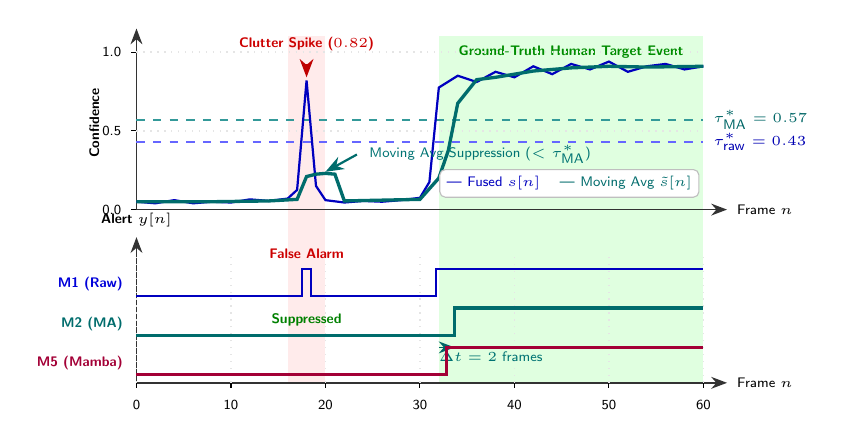
\begin{tikzpicture}[
    >=Stealth,
    font=\sffamily\scriptsize,
    axis/.style={draw=black!80, ->, semithick},
    gridl/.style={draw=black!10, dotted, line width=0.5pt},
    rawline/.style={draw=blue!75!black, thick},
    maline/.style={draw=teal!85!black, very thick},
    mambaline/.style={draw=purple!80!black, thick, dash pattern=on 3pt off 2pt},
    decision/.style={draw=red!80!black, line width=1.4pt},
    eventbg/.style={fill=green!12, draw=none}
]

% Coordinate dimensions:
% X-axis: 0 to 60 frames -> canvas X: 0 to 7.2 cm (scale: 0.12 cm/frame)
% Panel 1: Fused Confidence s[n] (Canvas Y: 2.2 to 4.2 cm)
% Panel 2: Decision Traces y[n] (Canvas Y: 0.0 to 1.5 cm)

% Shaded True Target Region (Frames 32 to 60 -> X: 3.84 to 7.2)
\fill[eventbg] (3.84, 0.0) rectangle (7.2, 4.4);
\node[font=\sffamily\tiny\bfseries, text=green!55!black, anchor=north] at (5.52, 4.4) {Ground-Truth Human Target Event};

% Shaded Distractor Spike Region (Frames 16 to 20 -> X: 1.92 to 2.4)
\fill[red!8] (1.92, 0.0) rectangle (2.4, 4.4);

% -------------------------------------------------------------
% TOP PANEL: Fused Confidence s[n] & Filter Responses
% -------------------------------------------------------------
\draw[axis] (0, 2.2) -- (7.5, 2.2) node[right, font=\sffamily\tiny] {Frame $n$};
\draw[axis] (0, 2.2) -- (0, 4.5);
\node[rotate=90, anchor=south, font=\sffamily\tiny\bfseries] at (-0.35, 3.3) {Confidence};

% Y-ticks
\draw (0, 2.2) -- (-2pt, 2.2) node[left, font=\sffamily\tiny] {0.0};
\draw (0, 3.2) -- (-2pt, 3.2) node[left, font=\sffamily\tiny] {0.5};
\draw (0, 4.2) -- (-2pt, 4.2) node[left, font=\sffamily\tiny] {1.0};
\draw[gridl] (0, 3.2) -- (7.2, 3.2);
\draw[gridl] (0, 4.2) -- (7.2, 4.2);

% Threshold lines
\draw[draw=blue!60, dashed, line width=0.7pt] (0, 3.06) -- (7.2, 3.06) node[right, font=\sffamily\tiny, text=blue!70!black] {$\tau_{\text{raw}}^*=0.43$};
\draw[draw=teal!80, dashed, line width=0.8pt] (0, 3.34) -- (7.2, 3.34) node[right, font=\sffamily\tiny, text=teal!80!black] {$\tau_{\text{MA}}^*=0.57$};

% Trace 1: Raw fused confidence s[n]
% Background frames 0-16: ~0.05
% Frame 18: sharp isolated spike to 0.82
% Frames 19-31: ~0.05
% Frames 32-60: sustained target ~0.80 - 0.94
\draw[rawline] 
    (0.00, 2.30) -- (0.24, 2.28) -- (0.48, 2.32) -- (0.72, 2.28) -- 
    (0.96, 2.30) -- (1.20, 2.29) -- (1.44, 2.33) -- (1.68, 2.31) -- 
    (1.92, 2.34) -- (2.04, 2.45) -- (2.16, 3.84) -- (2.28, 2.50) -- 
    (2.40, 2.32) -- (2.64, 2.29) -- (2.88, 2.31) -- (3.12, 2.30) -- 
    (3.36, 2.32) -- (3.60, 2.35) -- (3.72, 2.55) -- (3.84, 3.75) -- 
    (4.08, 3.90) -- (4.32, 3.82) -- (4.56, 3.95) -- (4.80, 3.88) -- 
    (5.04, 4.02) -- (5.28, 3.92) -- (5.52, 4.05) -- (5.76, 3.98) -- 
    (6.00, 4.08) -- (6.24, 3.95) -- (6.48, 4.02) -- (6.72, 4.05) -- 
    (6.96, 3.98) -- (7.20, 4.02);

% Trace 2: Moving average s_MA[n] (smoothed, suppresses frame 18 spike to ~0.16)
\draw[maline] 
    (0.00, 2.30) -- (0.96, 2.30) -- (1.68, 2.31) -- 
    (2.04, 2.33) -- (2.16, 2.62) -- (2.28, 2.65) -- (2.40, 2.66) -- (2.52, 2.65) -- (2.64, 2.31) -- 
    (3.60, 2.33) -- (3.84, 2.60) -- (3.96, 2.95) -- (4.08, 3.55) -- 
    (4.32, 3.85) -- (4.56, 3.88) -- (4.80, 3.92) -- (5.04, 3.96) -- 
    (5.52, 4.00) -- (6.00, 4.02) -- (6.48, 4.01) -- (7.20, 4.02);

% Annotation for noise spike vs smoothed
\draw[->, thick, red!75!black] (2.16, 4.05) -- (2.16, 3.88);
\node[font=\sffamily\tiny\bfseries, text=red!80!black, above=1pt] at (2.16, 4.05) {Clutter Spike ($0.82$)};

\draw[->, thick, teal!85!black] (2.8, 2.9) -- (2.4, 2.68);
\node[font=\sffamily\tiny, text=teal!90!black, right=1pt] at (2.8, 2.9) {Moving Avg Suppression ($< \tau_{\text{MA}}^*$)};

% -------------------------------------------------------------
% BOTTOM PANEL: Causal Binary Alert Decisions y[n] \in {0, 1}
% -------------------------------------------------------------
\draw[axis] (0, 0.0) -- (7.5, 0.0) node[right, font=\sffamily\tiny] {Frame $n$};
\draw[axis] (0, 0.0) -- (0, 1.85) node[above, font=\sffamily\tiny\bfseries] {Alert $y[n]$};

% Tick labels for frames
\foreach \f/\x in {0/0.0, 10/1.2, 20/2.4, 30/3.6, 40/4.8, 50/6.0, 60/7.2} {
    \draw (\x, 0.0) -- (\x, -2pt) node[below=1pt, font=\sffamily\tiny] {\f};
    \draw[gridl] (\x, 0.0) -- (\x, 1.6);
}

% M1 Trace (y-offset: 1.1)
\node[anchor=east, font=\sffamily\tiny\bfseries, text=blue!85!black] at (-0.05, 1.25) {M1 (Raw)};
\draw[blue!75!black, thick] (0, 1.1) -- (2.10, 1.1) -- (2.10, 1.45) -- (2.22, 1.45) -- (2.22, 1.1) -- (3.80, 1.1) -- (3.80, 1.45) -- (7.2, 1.45);
\node[font=\sffamily\tiny, text=red!80!black, anchor=south] at (2.16, 1.45) {\textbf{False Alarm}};

% M2 Trace (y-offset: 0.6)
\node[anchor=east, font=\sffamily\tiny\bfseries, text=teal!85!black] at (-0.05, 0.75) {M2 (MA)};
\draw[teal!85!black, line width=1.3pt] (0, 0.6) -- (4.04, 0.6) -- (4.04, 0.95) -- (7.2, 0.95);
\node[font=\sffamily\tiny, text=green!50!black, anchor=south] at (2.16, 0.6) {\textbf{Suppressed}};
\draw[->, semithick, teal!80!black] (3.84, 0.45) -- (4.04, 0.45);
\node[font=\sffamily\tiny, text=teal!90!black, anchor=north] at (4.50, 0.52) {$\Delta t = 2\text{ frames}$};

% M5 Trace (y-offset: 0.1)
\node[anchor=east, font=\sffamily\tiny\bfseries, text=purple!85!black] at (-0.05, 0.25) {M5 (Mamba)};
\draw[purple!85!black, line width=1.1pt] (0, 0.1) -- (3.94, 0.1) -- (3.94, 0.45) -- (7.2, 0.45);

% Legend box
\node[draw=black!25, fill=white, rounded corners=2pt, font=\sffamily\tiny, anchor=south east, inner sep=2.5pt] at (7.15, 2.35) {
    \textcolor{blue!75!black}{\textbf{---} Fused $s[n]$} \quad
    \textcolor{teal!85!black}{\textbf{---} Moving Avg $\tilde{s}[n]$}
};

\end{tikzpicture}
}
\caption{Temporal confidence trace (top) and causal alert decisions (bottom) across clutter and target events.}
\label{fig:real_temporal_sequence}
\end{figure}

\begin{figure}[!t]
\centering
\resizebox{0.88\columnwidth}{!}{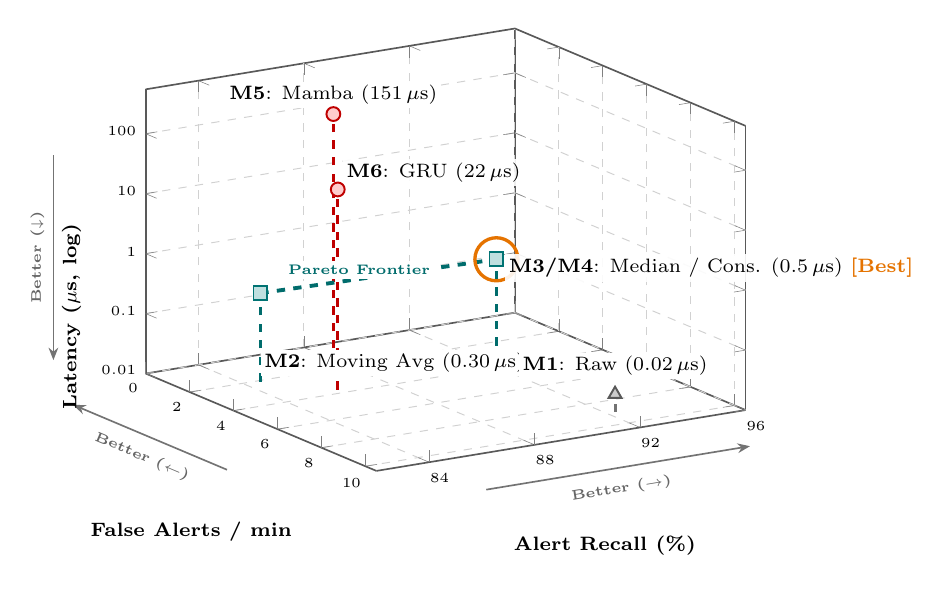
\begin{tikzpicture}
\begin{axis}[
  width=9.2cm,
  height=7.2cm,
  view={58}{22},
  xmin=0, xmax=10.5,
  ymin=82, ymax=96,
  zmode=log,
  zmin=0.01, zmax=550,
  zminorticks=false,
  xtick={0, 2, 4, 6, 8, 10},
  ytick={84, 88, 92, 96},
  ztick={0.01, 0.1, 1, 10, 100},
  zticklabels={$0.01$, $0.1$, $1$, $10$, $100$},
  xlabel={\textbf{False Alerts / min}},
  ylabel={\textbf{Alert Recall (\%)}},
  zlabel={\textbf{Latency ($\mu\text{s}$, log)}},
  xlabel style={font=\scriptsize, yshift=-10pt},
  ylabel style={font=\scriptsize, yshift=-14pt},
  zlabel style={font=\scriptsize, xshift=-34pt},
  tick label style={font=\tiny},
  axis line style={semithick, black!65},
  grid=major,
  grid style={line width=0.35pt, draw=black!18, dashed},
  clip=false
]

  % 1. Directional Improvement Arrows
  \draw[-{Stealth[length=4.5pt, width=3.5pt]}, semithick, black!55] 
    (axis cs:8.5, 78.0, 0.01) -- (axis cs:1.5, 78.0, 0.01)
    node[pos=0.5, sloped, below=1.5pt, font=\tiny\bfseries, text=black!60] {Better ($\leftarrow$)};

  \draw[-{Stealth[length=4.5pt, width=3.5pt]}, semithick, black!55, yshift=-4pt] 
    (axis cs:12.5, 84.5, 0.01) -- (axis cs:12.5, 94.5, 0.01)
    node[pos=0.5, sloped, below=1.5pt, font=\tiny\bfseries, text=black!60] {Better ($\rightarrow$)};

  \draw[{Stealth[length=4.5pt, width=3.5pt]}-, semithick, black!55] 
    (axis cs:0, 78.5, 0.03) -- (axis cs:0, 78.5, 80.0)
    node[pos=0.5, sloped, above=2pt, font=\tiny\bfseries, text=black!60, fill=white, inner sep=1pt] {Better ($\downarrow$)};

  % 2. Depth Drop Lines
  \draw[dashed, black!55,     line width=1.1pt] (axis cs:9.0, 92.3, 0.01) -- (axis cs:9.0, 92.3, 0.02);
  \draw[dashed, teal!85!black, line width=1.1pt] (axis cs:2.1, 84.6, 0.01) -- (axis cs:2.1, 84.6, 0.30);
  \draw[dashed, teal!85!black, line width=1.1pt] (axis cs:3.6, 92.3, 0.01) -- (axis cs:3.6, 92.3, 0.52);
  \draw[dashed, red!75!black,  line width=1.1pt] (axis cs:3.7, 86.2, 0.01) -- (axis cs:3.7, 86.2, 21.8);
  \draw[dashed, red!75!black,  line width=1.1pt] (axis cs:1.7, 87.7, 0.01) -- (axis cs:1.7, 87.7, 150.6);

  % 3. Sub-Microsecond Pareto Frontier
  \addplot3[
    color=teal!85!black,
    line width=1.4pt,
    dashed
  ] coordinates {
    (2.1, 84.6, 0.30)
    (3.6, 92.3, 0.52)
  };

  \node[font=\tiny\bfseries, text=teal!85!black, fill=white, inner sep=1.5pt, sloped, above] 
    at (axis cs:2.75, 87.8, 0.38) {Pareto Frontier};

  % 4. Method Markers & Annotations
  \addplot3[
    only marks,
    mark=square*,
    mark size=2.5pt,
    draw=teal!90!black,
    fill=teal!25,
    line width=0.7pt
  ] coordinates {
    (2.1, 84.6, 0.30)
    (3.6, 92.3, 0.52)
  };

  \node[
    draw=orange!90!black,
    line width=1.2pt,
    circle,
    inner sep=5.5pt
  ] at (axis cs:3.6, 92.3, 0.52) {};

  \node[font=\scriptsize, anchor=north west, fill=white, inner sep=1.2pt] 
    at (axis cs:2.1, 84.6, 0.035) {\textbf{M2}: Moving Avg ($0.30\,\mu\text{s}$)};

  \node[font=\scriptsize, anchor=west, fill=white, fill opacity=0.9, text opacity=1, inner sep=1.5pt] 
    at (axis cs:3.95, 92.3, 0.42) {\textbf{M3/M4}: Median / Cons. ($0.5\,\mu\text{s}$) \textbf{\textcolor{orange!90!black}{[Best]}}};

  \addplot3[
    only marks,
    mark=*,
    mark size=2.5pt,
    draw=red!75!black,
    fill=red!20,
    line width=0.7pt
  ] coordinates {
    (1.7, 87.7, 150.6)
    (3.7, 86.2, 21.8)
  };

  \node[font=\scriptsize, anchor=south, fill=white, inner sep=1.2pt] 
    at (axis cs:1.7, 87.7, 185.0) {\textbf{M5}: Mamba ($151\,\mu\text{s}$)};

  \node[font=\scriptsize, anchor=south west, fill=white, fill opacity=0.9, text opacity=1, inner sep=1.4pt] 
    at (axis cs:3.9, 86.2, 26.0) {\textbf{M6}: GRU ($22\,\mu\text{s}$)};

  \addplot3[
    only marks,
    mark=triangle*,
    mark size=2.7pt,
    draw=black!65,
    fill=black!20,
    line width=0.7pt
  ] coordinates {
    (9.0, 92.3, 0.02)
  };

  \node[font=\scriptsize, anchor=south, fill=white, inner sep=1.2pt] 
    at (axis cs:9.0, 92.3, 0.035) {\textbf{M1}: Raw ($0.02\,\mu\text{s}$)};

\end{axis}
\end{tikzpicture}}
\caption{Operational trade-offs across causal temporal decision methods. Log-scale $z$-axis encodes filter runtime ($\mu$s).}
\label{fig:performance_tradeoff}
\end{figure}

\begin{table*}[t]
\centering
\caption{Benchmark of Causal Temporal Decision Methods on Held-Out Test Sequences ($W = 5$, 166.7~ms Span, 24~Hz)}
\label{tab:postprocessing_benchmark}
\resizebox{\textwidth}{!}{%
\begin{tabular}{lcccccc}
\toprule
\textbf{Decision Method} & \textbf{$\tau^*$} & \textbf{Alert Recall (Tile [95\% CI] / Parent)} & \textbf{Frame $F_1$-Score [95\% CI]} & \textbf{False Alerts / min} & \textbf{Alert Latency (Time-to-Alarm)} & \textbf{Filter Runtime / Frame} \\
\midrule
M1: Baseline Raw Thresholding          & 0.43 & \textbf{92.3\% (12/13) [76.9, 100.0] / 8/9} & 0.813 [0.635, 0.924]          & 9.0                         & \textbf{188.9 ms (4.5 frames)}  & \textbf{0.02 $\mu$s ($O(1)$, 0 B state)} \\
M2: Five-Frame Moving Average          & 0.57 & 84.6\% (11/13) [61.5, 100.0] / 8/9          & 0.781 [0.576, 0.912]          & 2.1$^\dagger$               & 592.3 ms (14.2 frames)          & 0.30 $\mu$s ($O(1)$, 20 B state) \\
M3: Five-Frame Median Filter           & 0.49 & \textbf{92.3\% (12/13) [76.9, 100.0] / 8/9} & 0.805 [0.615, 0.925]          & 3.6                         & 291.7 ms (7.0 frames)           & 0.42 $\mu$s ($O(W)$, 20 B state) \\
M4: Five-Frame History Consensus       & 0.49 & \textbf{92.3\% (12/13) [76.9, 100.0] / 8/9} & 0.802 [0.613, 0.921]          & 3.6                         & 313.9 ms (7.5 frames)           & 0.63 $\mu$s ($O(W)$, 5 B state) \\
M5: Learned Mamba-SSSM (5 seeds)       & 0.73 & 87.7\% $\pm$ 4.2\% / 8/9                     & 0.717 $\pm$ 0.040 [0.501, 0.863] & \textbf{1.7 $\pm$ 0.6}     & 587.5 ms (14.1 frames)          & 150.59 $\mu$s ($O(d_{\text{model}}d_{\text{state}})$, 512 B) \\
M6: Learned GRU Baseline (5 seeds)     & 0.50 & 86.2\% $\pm$ 3.4\% / 8/9                     & \textbf{0.822 $\pm$ 0.007 [0.642, 0.933]} & 3.7 $\pm$ 0.3  & 577.3 ms (13.9 frames)          & 21.80 $\mu$s ($O(d_{\text{hidden}}^2)$, 64 B) \\
\bottomrule
\multicolumn{7}{l}{\footnotesize Bold indicates best metric in column. Alert recall reports tile recall (with 95\% bootstrap confidence intervals [CIs], $N=13$ positive tiles) and parent-video recall ($N=9$ positive parents). Frame $F_1$ CIs: percentile bootstrap over the 24 test clips ($B=1000$) of the pooled frame $F_1$; for M5/M6, the mean of the per-seed CIs.} \\
\multicolumn{7}{l}{\footnotesize $^\dagger$All learned-vs-classical comparisons show no statistically significant gain after Holm-Bonferroni correction ($p > 0.39$ at parent-video level; Section~V-C). Denominators: 13 positive tiles, 9 positive parents, 3.868 min flight time (5,570 frames).}
\end{tabular}%
}
\end{table*}

\subsection{Two Operating Points: False-Alert Suppression versus Recall Preservation}
Across the test split, causal filtering provides two practical operating points depending on mission priorities (Table~\ref{tab:postprocessing_benchmark}, Fig.~\ref{fig:performance_tradeoff}). Although the moving average filter (M2) has lower tile recall than raw thresholding (84.6\% vs.\ 92.3\%), this difference is only one missed tile (11/13 vs.\ 12/13), yielding overlapping 95\% bootstrap confidence intervals. At the parent-video level, all classical methods achieve identical 88.9\% recall (8/9 videos), as the tile missed by M2 is alerted in its sibling crop.

When suppressing false alerts is the priority, the moving average (M2) cuts false alerts by 77\%, from 9.0 to 2.1 per minute (65.3\% false alarm suppression ratio [FASR]), reducing false-positive frames from 75 to 26 over the 3.87-min test. Paired Wilcoxon signed-rank tests confirm significant reductions in false-positive frames ($W=2.0$, $p=0.0056$) and false-alert events ($W=2.0$, $p=0.0087$) compared to raw thresholding, with alert latency of 592.3~ms.

When preserving recall is the priority, median filtering (M3) and consensus (M4) retain full baseline recall (92.3\% tile, 88.9\% parent). They reduce false alerts by 60\% (to 3.6 per minute, 32.0\% FASR) with faster response (291.7~ms vs.\ 592.3~ms). Because median filtering preserves sharp signal transitions, M3 confirms targets quickly while suppressing transient single-frame clutter spikes.

\subsection{Learned Sequence Models: False-Alert Reduction and Edge Trade-Offs}
Learned sequence models perform strongly in false-alert suppression and alert recall (Table~\ref{tab:postprocessing_benchmark}). Mamba-SSSM (M5) achieves the lowest false-alert rate in the benchmark at 1.7 alerts per minute (an 81.1\% reduction vs.\ raw thresholding), while maintaining 87.7\% tile recall and 88.9\% parent-video recall (8/9 videos). Compared to the low-false-alert moving average (M2, 84.6\% tile recall), Mamba achieves both higher alert recall and fewer false alerts. Similarly, the GRU baseline (M6) achieves 86.2\% tile recall with 3.7 false alerts per minute (comparable to median filtering's 3.6) and reaches the highest overall frame-level $F_1\text{-score}$ ($0.822 \pm 0.007$). Both learned models reliably preserve parent-level alert recall (8/9 videos).

While learned models incur slightly higher alert latency (~580~ms vs.\ 291.7~ms for median), this delay is minor in real missions; a half-second confirmation does not cause the drone to fly past the target. Furthermore, the per-frame filter runtime gap ($0.30\,\mu\text{s}$ for M2 vs.\ $21.80\,\mu\text{s}$ for GRU and $150.59\,\mu\text{s}$ for Mamba) is practically negligible. Against the 41.7~ms frame budget (24~Hz), even the slowest filter takes roughly 0.4\% of available time, while YOLO11n inference consumes over 98\% ($10.2\text{ ms}$). Filter latency is therefore not a limiting constraint. Instead, the primary edge trade-offs are memory footprint and training requirements: Mamba requires a 512~B recurrent state and 753 parameters, and GRU requires 64~B state and 1,681 parameters, compared to only 20~B buffer, zero parameters, and no training data for classical filters. When memory allows, learned sequence models deliver effective false-alert suppression with high recall.

\subsection{Environmental Robustness Across Biomes}
Table~\ref{tab:per_biome_benchmark} reports performance across the three test biomes (8 tiles per biome, 5,570 frames total). Because biomes contain 4 or 5 positive sequences, recall percentages correspond to small counts: 75.0\% in forest is 3/4 detected tiles, and 80.0\% in snow is 4/5 tiles. Across all biomes, moving average filtering (M2) substantially lowers false alerts compared to raw thresholding (M1): desert drops by 85.7\% (10.50 to 1.50 FA/min); forest drops by 73.3\% (12.49 to 3.33 FA/min); and snow drops by 66.7\% (4.50 to 1.50 FA/min). Although smoothing causes M2 to miss one tile under dense forest (3/4 vs.\ 4/4 for M3), M2 achieves the lowest false-alert rate in each biome.

\begin{table}[!t]
\centering
\caption{Biome-Stratified Causal Decision Performance on Held-Out Test Split}
\label{tab:per_biome_benchmark}
\resizebox{\columnwidth}{!}{%
\begin{tabular}{llcccc}
\toprule
\textbf{Environment} & \textbf{Decision Method} & \textbf{$\tau^*$} & \textbf{Alert Recall (\%)} & \textbf{FA / min} & \textbf{FP Frames} \\
\midrule
\textbf{Arid Desert} (1.33 min)
  & M1: Raw Baseline        & 0.43 & 100.0\% (4/4) & 10.50 & 32 \\
  & M2: Moving Average      & 0.57 & 100.0\% (4/4) & \textbf{1.50} & \textbf{10} \\
  & M3: Median Filter       & 0.49 & 100.0\% (4/4) & 3.00 & 20 \\
  & M4: History Consensus   & 0.49 & 100.0\% (4/4) & 3.00 & 20 \\
\midrule
\textbf{Temperate Forest} (1.20 min)
  & M1: Raw Baseline        & 0.43 & 100.0\% (4/4) & 12.49 & 34 \\
  & M2: Moving Average      & 0.57 & 75.0\% (3/4)  & \textbf{3.33} & \textbf{13} \\
  & M3: Median Filter       & 0.49 & 100.0\% (4/4) & 4.99 & 21 \\
  & M4: History Consensus   & 0.49 & 100.0\% (4/4) & 4.99 & 21 \\
\midrule
\textbf{Snow/Alpine} (1.33 min)
  & M1: Raw Baseline        & 0.43 & 80.0\% (4/5)  & 4.50 & 9 \\
  & M2: Moving Average      & 0.57 & 80.0\% (4/5)  & \textbf{1.50} & \textbf{3} \\
  & M3: Median Filter       & 0.49 & 80.0\% (4/5)  & 3.00 & 10 \\
  & M4: History Consensus   & 0.49 & 80.0\% (4/5)  & 3.00 & 10 \\
\bottomrule
\end{tabular}%
}
\end{table}

\subsection{Temporal Window Length Sensitivity}
On validation sequences, testing window lengths $W \in \{1, 3, 5, 7\}$ illustrates the trade-off between false-alert reduction and alert delay. A single-frame window ($W=1$) produces frequent noise spikes (22.8 FA/min, $F_1 = 0.849$). Increasing window size to $W=3$ (83.3~ms span) and $W=5$ (166.7~ms span) lowers false alerts to 15.3 and 8.4 per minute. A window of $W=7$ (250.0~ms span) achieves 5.8 FA/min but adds latency. On test sequences, moving average false alerts decrease from 4.65 ($W=1$) to 2.07 ($W=5$) per minute. Similarly, median filtering lowers false alerts from 5.69 to 3.62 per minute while maintaining 92.3\% recall across $W \in \{1, 3, 5\}$. Thus, $W=5$ balances fast alerting and false-alarm suppression.

\subsection{Limitations}
Several limitations apply to this study. First, a key limitation is the small test set (24 tiles, 13 positive targets across 3.87~min of flight); missing one target shifts tile recall by 7.7\%, though parent-video recall is 88.9\%. Second, the pseudo-TIR channel is generated from RGB frames using a 256-level lookup table, evaluating correlated representations rather than radiometric thermal data ($8\text{--}14\,\mu\text{m}$); physical wavelength sensitivity cannot be evaluated from RGB luminance remapping. Third, sequence models were compact architectures (753 to 1,681 parameters) trained on scalar confidences. Fourth, video streams were synthetic, omitting aerodynamic turbulence. Finally, benchmarks reflect desktop hardware.

\subsection{Sensitivity Analysis: Recall-Weighted Operational Regimes}
\label{sec:sensitivity_analysis}
In life-critical search missions, doctrines often prioritize catching every target over avoiding false alarms. We evaluate two separate recall-weighted formulations (Eq.~\eqref{eq:fbeta}) with validation precision floor $P \ge 0.95$: harmonic $F_2\text{-score}$ ($\tau^*_{F_2}$) and asymmetric misclassification cost ($\tau^*_{C}$) penalizing false negatives $5\times$ over false alarms. Calibrating each independently on validation sequences identifies identical sensitive threshold regimes ($\tau^* \in [0.13, 0.19]$, Table~\ref{tab:f2_sensitivity}). When thresholds are lowered for faint targets, raw thresholding false alerts jump from 9.0 to 21.97 per minute. In contrast, causal filters smooth out these spikes: moving average limits false alerts to 9.57 per minute, while median filtering and consensus keep false alerts to ~8.1 per minute (63.5\% reduction vs.\ raw). Temporal filtering thus stabilizes sensitive operating thresholds under both criteria without excessive clutter alerts.

\begin{table}[!t]
\centering
\caption{Recall-Weighted ($F_2$, Asymmetric Cost) vs.\ Baseline Operating Points}
\label{tab:f2_sensitivity}
\resizebox{\columnwidth}{!}{%
\begin{tabular}{lcccccc}
\toprule
\textbf{Method} & \textbf{$\tau^*$} & \textbf{Base Rec.} & \textbf{$F_2$ Rec.} & \textbf{FA/min} & \textbf{$\Delta$FA/min} & \textbf{Delay (ms)} \\
\midrule
M1: Raw Thresholding     & 0.19 & 92.3\% & 100.0\% & 21.97 & +12.97 & 267.2 \\
M2: Moving Average       & 0.15 & 84.6\% & 92.3\%  & 9.57  & +7.47  & 91.1 \\
M3: Median Filter        & 0.13 & 92.3\% & 92.3\%  & 8.27  & +4.67  & 99.0 \\
M4: History Consensus    & 0.13 & 92.3\% & 92.3\%  & 8.01  & +4.41  & 119.8 \\
\bottomrule
\end{tabular}%
}
\end{table}

\balance

\section{Conclusion}
This paper investigated causal temporal decision strategies to convert noisy dual-stream visible and pseudo-thermal detections into reliable search and rescue alerts. Holding upstream YOLO11n detectors and the late-fusion max gate fixed, we benchmarked six causal decision methods under fixed per-method thresholds, focusing on false-alert suppression, alert recall, and memory footprint. Learned sequence models achieve the strongest overall false-alert reduction: Mamba-SSSM delivers the lowest false-alert rate across all methods (1.7 FA/min with 87.7\% tile recall and 88.9\% parent recall), while the GRU baseline achieves 86.2\% tile recall and the highest frame-level $F_1\text{-score}$. Training-free causal filters provide competitive alternatives: a five-frame moving average cuts false alerts by 77\% to 2.1 per minute at 84.6\% tile recall, and a five-frame median filter preserves 92.3\% tile recall with 3.6 false alerts per minute. Because filter execution takes less than 0.4\% of the 41.7~ms frame budget, filter latency is negligible for real-time tracking. The primary trade-off on edge avionics is memory footprint (512~B recurrent state vs.\ 20~B buffer) and training overhead. Simple causal filtering offers an efficient, training-free baseline, while learned sequence models provide maximum false-alarm suppression when memory allows. Future work will test these methods on real RGB-thermal datasets and embedded UAV hardware (such as the NVIDIA Jetson Orin Nano) during live flight trials.

\section*{AI Disclosure \& Code Availability}
Generative artificial intelligence (AI) tools (Gemini 3.8 Flash, Grok) were used for synthetic video generation and manuscript editing. Simulation frameworks, split manifests, and PyTorch implementations are publicly available at: \url{https://github.com/IamOumarIbrahim/multi-modal-detection}.

\bibliographystyle{IEEEtran}
\bibliography{references}

\end{document}
